\documentclass[
	letterpaper, % Paper size, specify a4paper (A4) or letterpaper (US letter)
	10pt, % Default font size, specify 10pt, 11pt or 12pt
]{CSUniSchoolLabReport}

%----------------------------------------------------------------------------------------
%	REPORT INFORMATION
%----------------------------------------------------------------------------------------

\title{Experiment Four\\ Fundamentals of Electromagnetics Lab \\ EECE2530/1} % Report title

\author{Michael \textsc{Brodskiy}\\ \small \href{mailto:Brodskiy.M@Northeastern.edu}{Brodskiy.M@Northeastern.edu}}

\date{November 1, 2023} % Date of the report

%----------------------------------------------------------------------------------------


\begin{document}

\maketitle % Insert the title, author and date using the information specified above

\begin{center}
	\begin{tabular}{l r}
		Date Performed: & October 18, 2023 \\ % Date the experiment was performed
        Partners: & Manas \textsc{Mahajan} \& Priyam \textsc{Modi} \\ % Partner names
		Instructor: & Professor \textsc{Marengo-Fuentes} \\ % Instructor/supervisor
        TAs: & Nicolas \textsc{Casilli} \& Farah \textsc{Ben Ayed} \\ % Teachers Assistants 
	\end{tabular}
\end{center}

\newpage

\begin{abstract}

  The goal of this laboratory experiment is to utilize the CST Studio Suite to design and simulate the properties of various devices. For this experiment, two devices will be fabricated and tested: a micro-strip transmission line and resonator.

\end{abstract}

\begin{flushleft}

  \textsc{Keywords:} \underline{CST Studio Suite}, \underline{simulate}, \underline{fabricate}, \underline{micro-strip}, \underline{transmission line}, \underline{resonator}

\end{flushleft}

\newpage

\section{Equipment}

\hspace{.5 in} Available equipment included:\\

\begin{itemize}

  \item CST Studio Suite

\end{itemize}

\section{Introduction \& Objectives}

We began the lab by setting up the construction and simulation environment within CST. After setting up the environment, the first device to be constructed is a micro-strip transmission line. Copper and aluminum were used as the conductive and dielectric elements. Field monitors were then set up to simulate the fields on the edges of the resonator. In a similar fashion, a micro-strip resonator was constructed, and plots for $S_{11}$ and $S_{21}$ were constructed.

\section{Results \& Analysis} 

For the transmission line, several simulations were run to generate Figures \ref{fig:1}-\ref{fig:12}, which include all $S$ parameters, electric fields, and magnetic fields. The results can be seen below:

\begin{figure}[H]
  \centering
  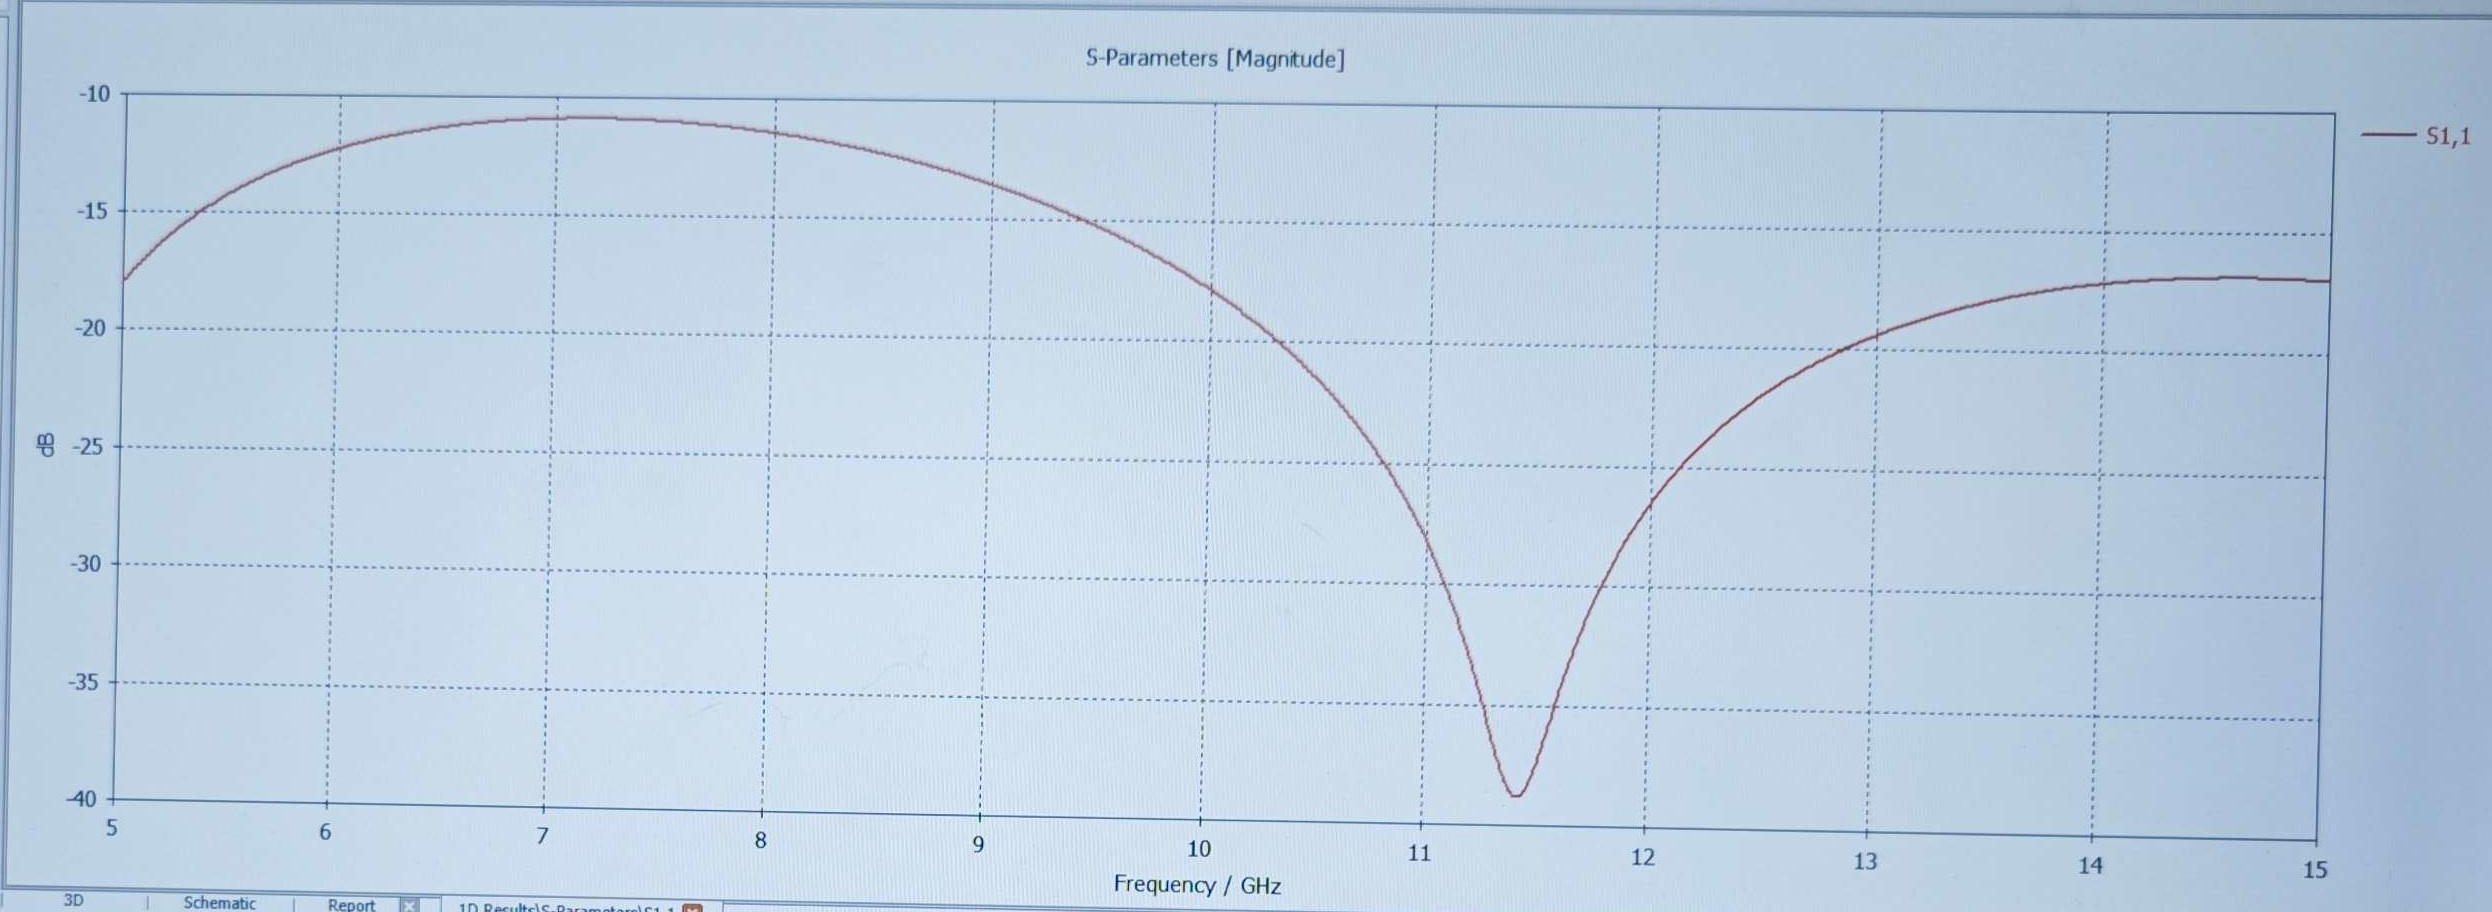
\includegraphics[width=.9\textwidth]{Figures/Lab Four/Line_S11.jpg}
  \caption{$S_{11}$ Parameter for the Transmission Line}
  \label{fig:1}
\end{figure}

\begin{figure}[H]
  \centering
  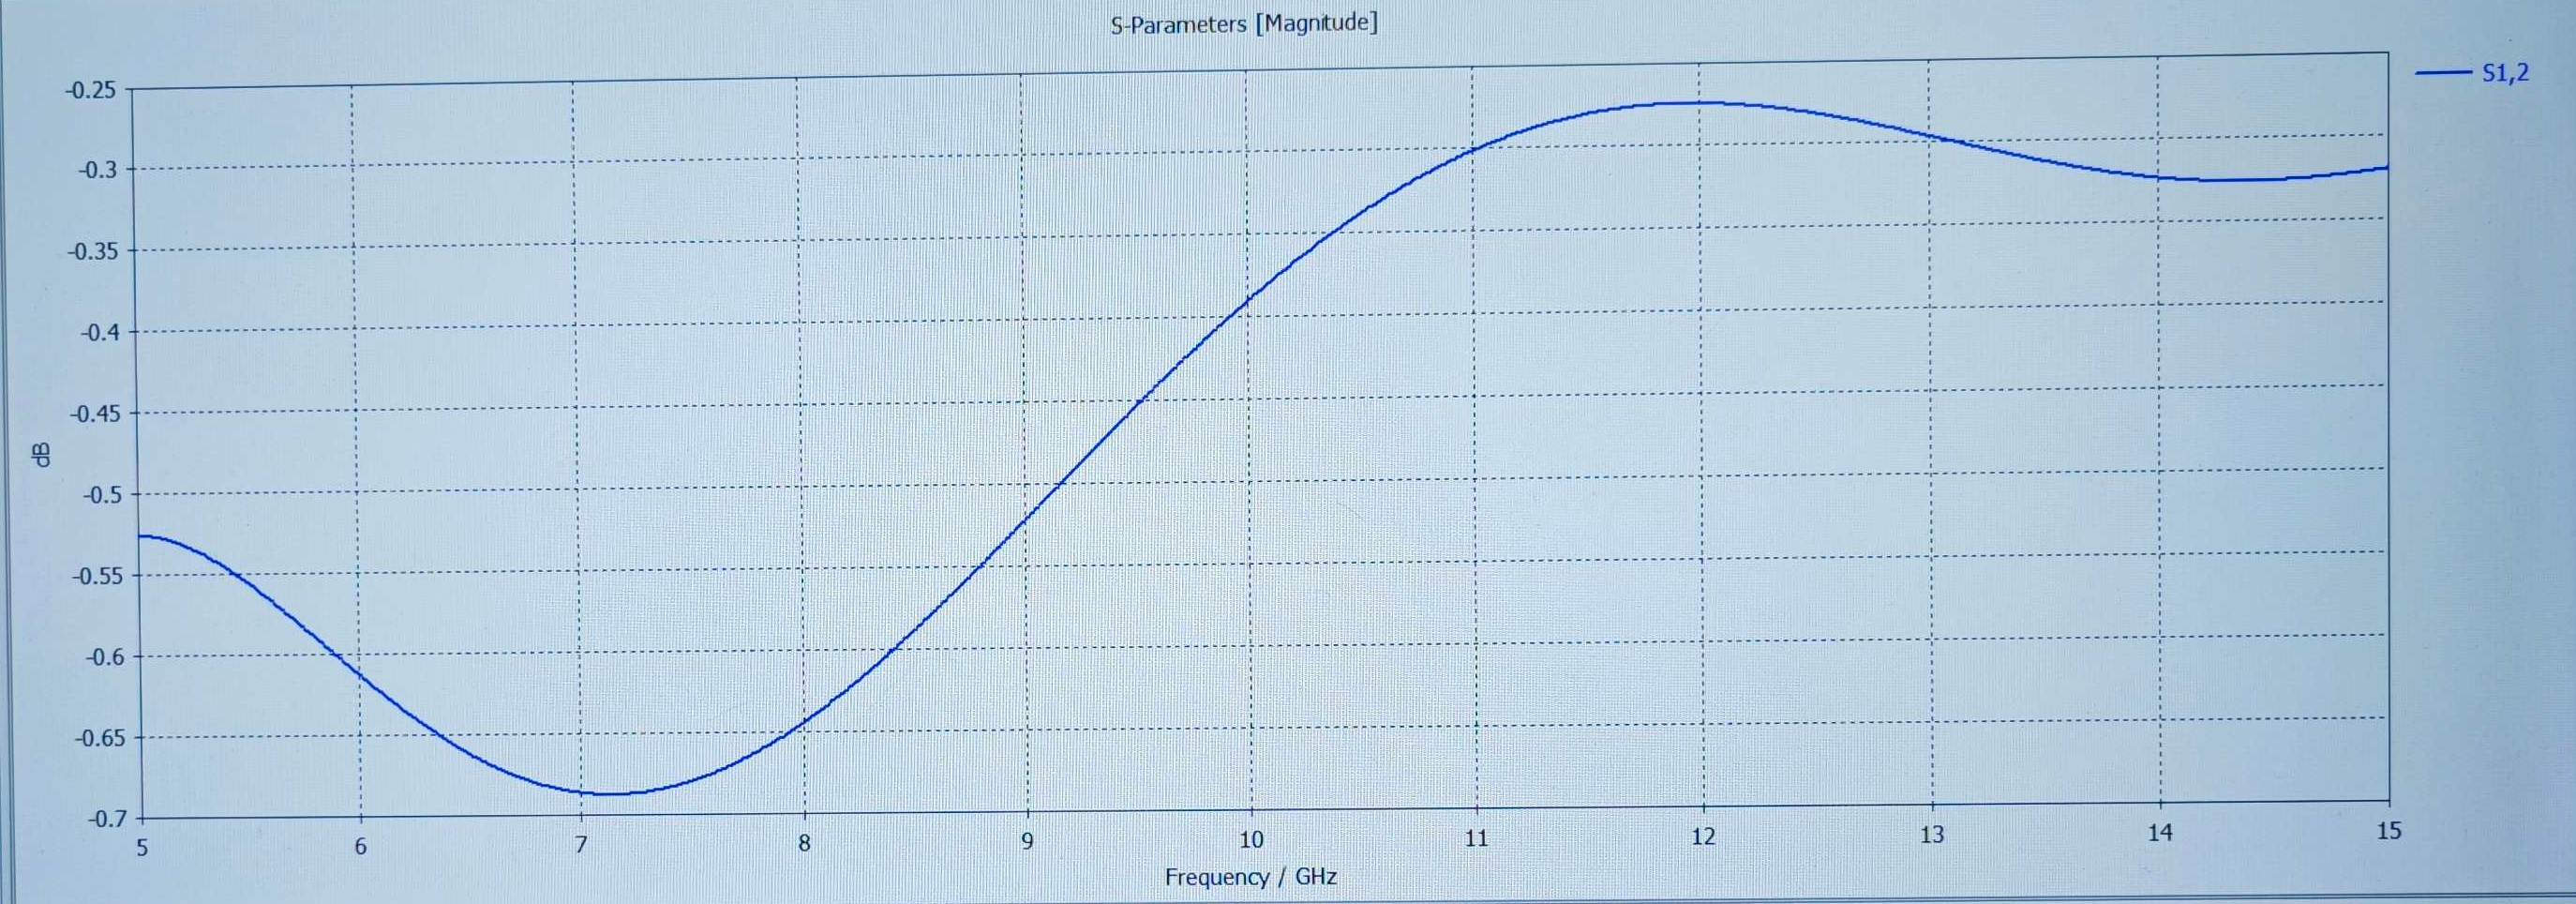
\includegraphics[width=.9\textwidth]{Figures/Lab Four/Line_S12.jpg}
  \caption{$S_{12}$ Parameter for the Transmission Line}
  \label{fig:2}
\end{figure}

\begin{figure}[H]
  \centering
  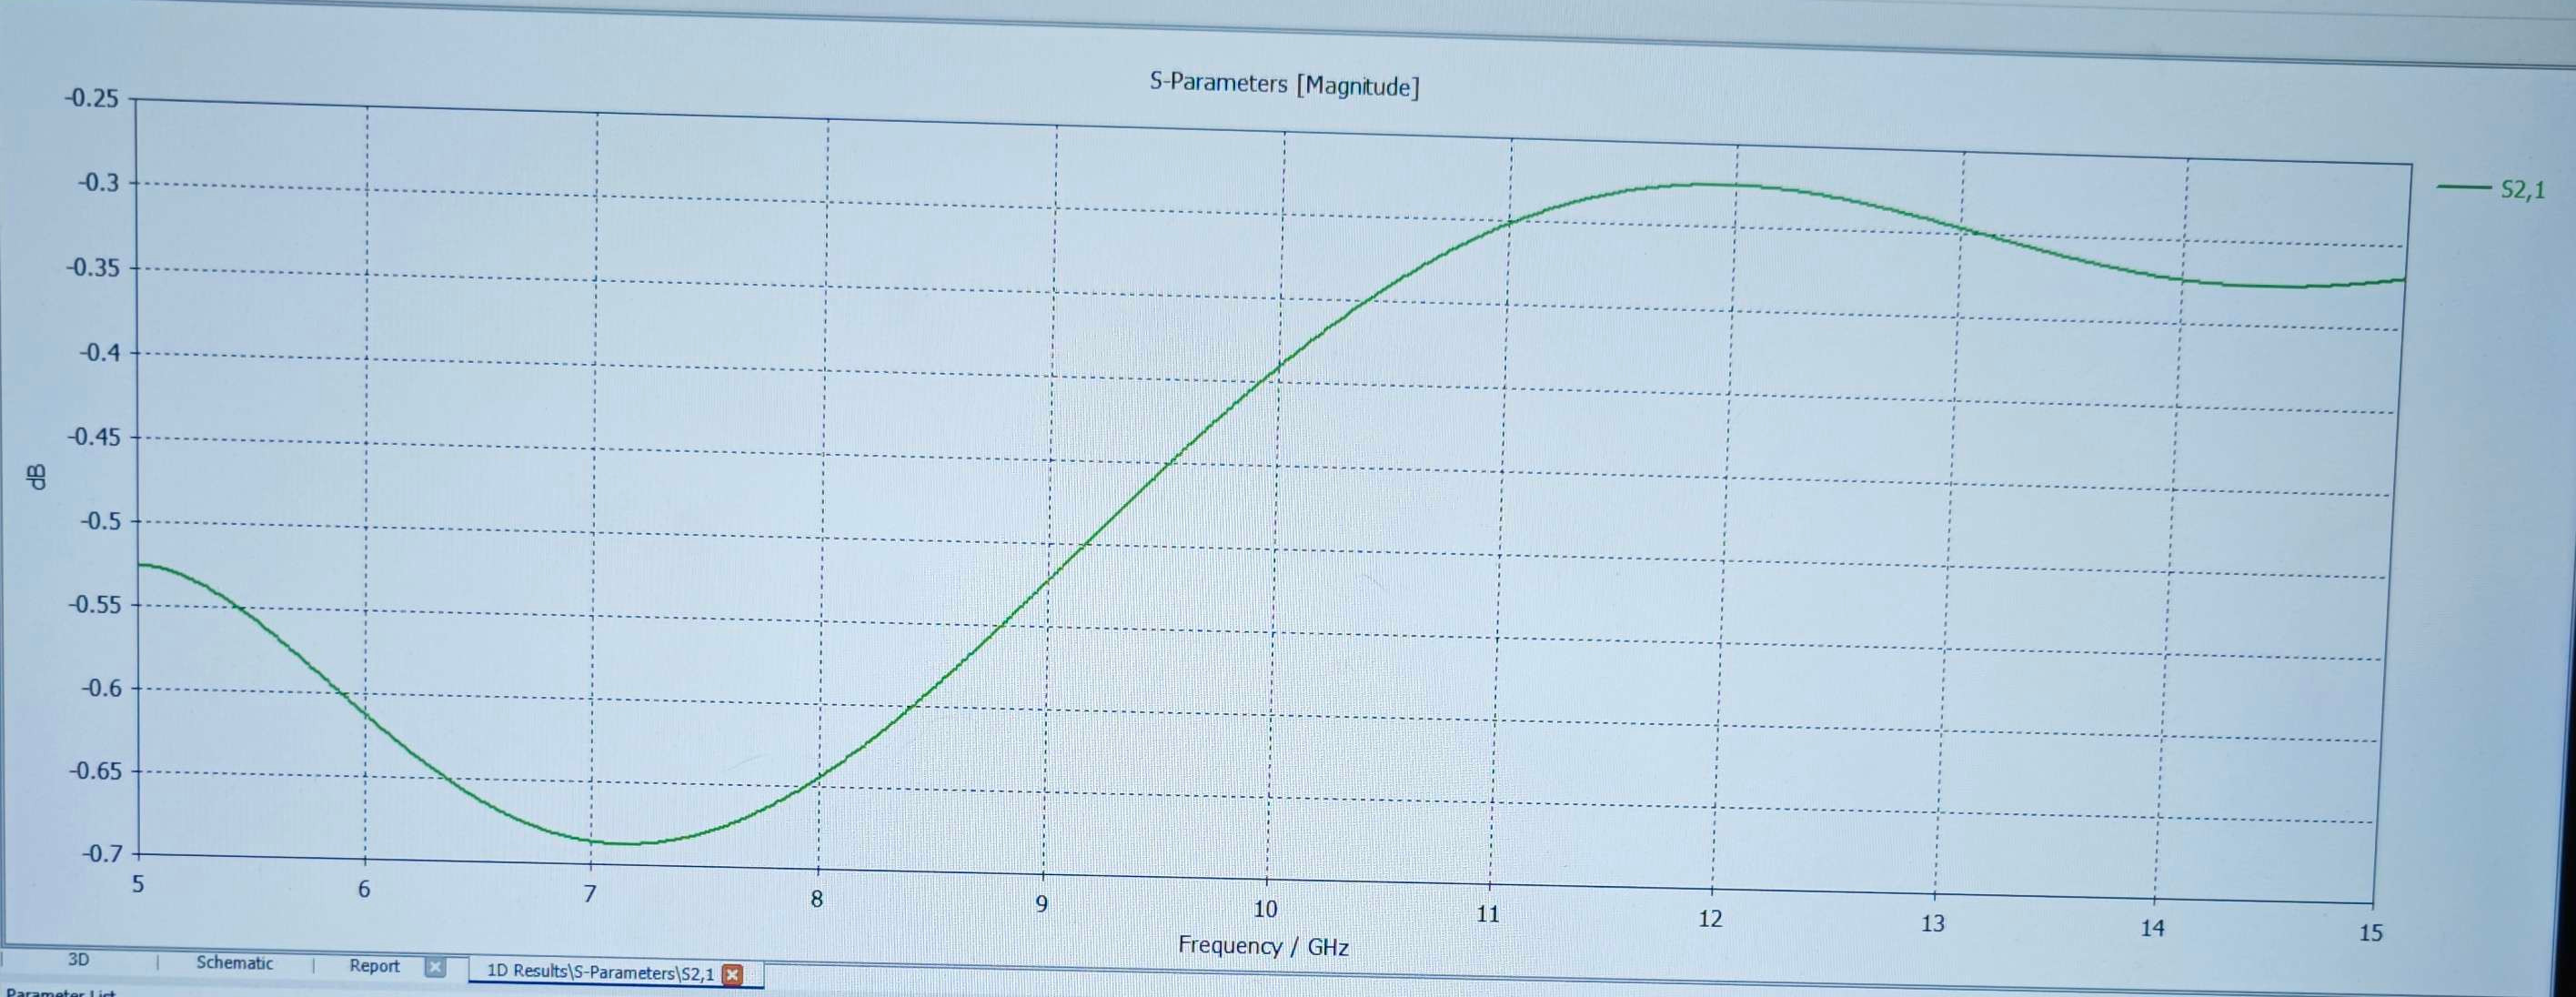
\includegraphics[width=.9\textwidth]{Figures/Lab Four/Line_S21.jpg}
  \caption{$S_{21}$ Parameter for the Transmission Line}
  \label{fig:3}
\end{figure}

\begin{figure}[H]
  \centering
  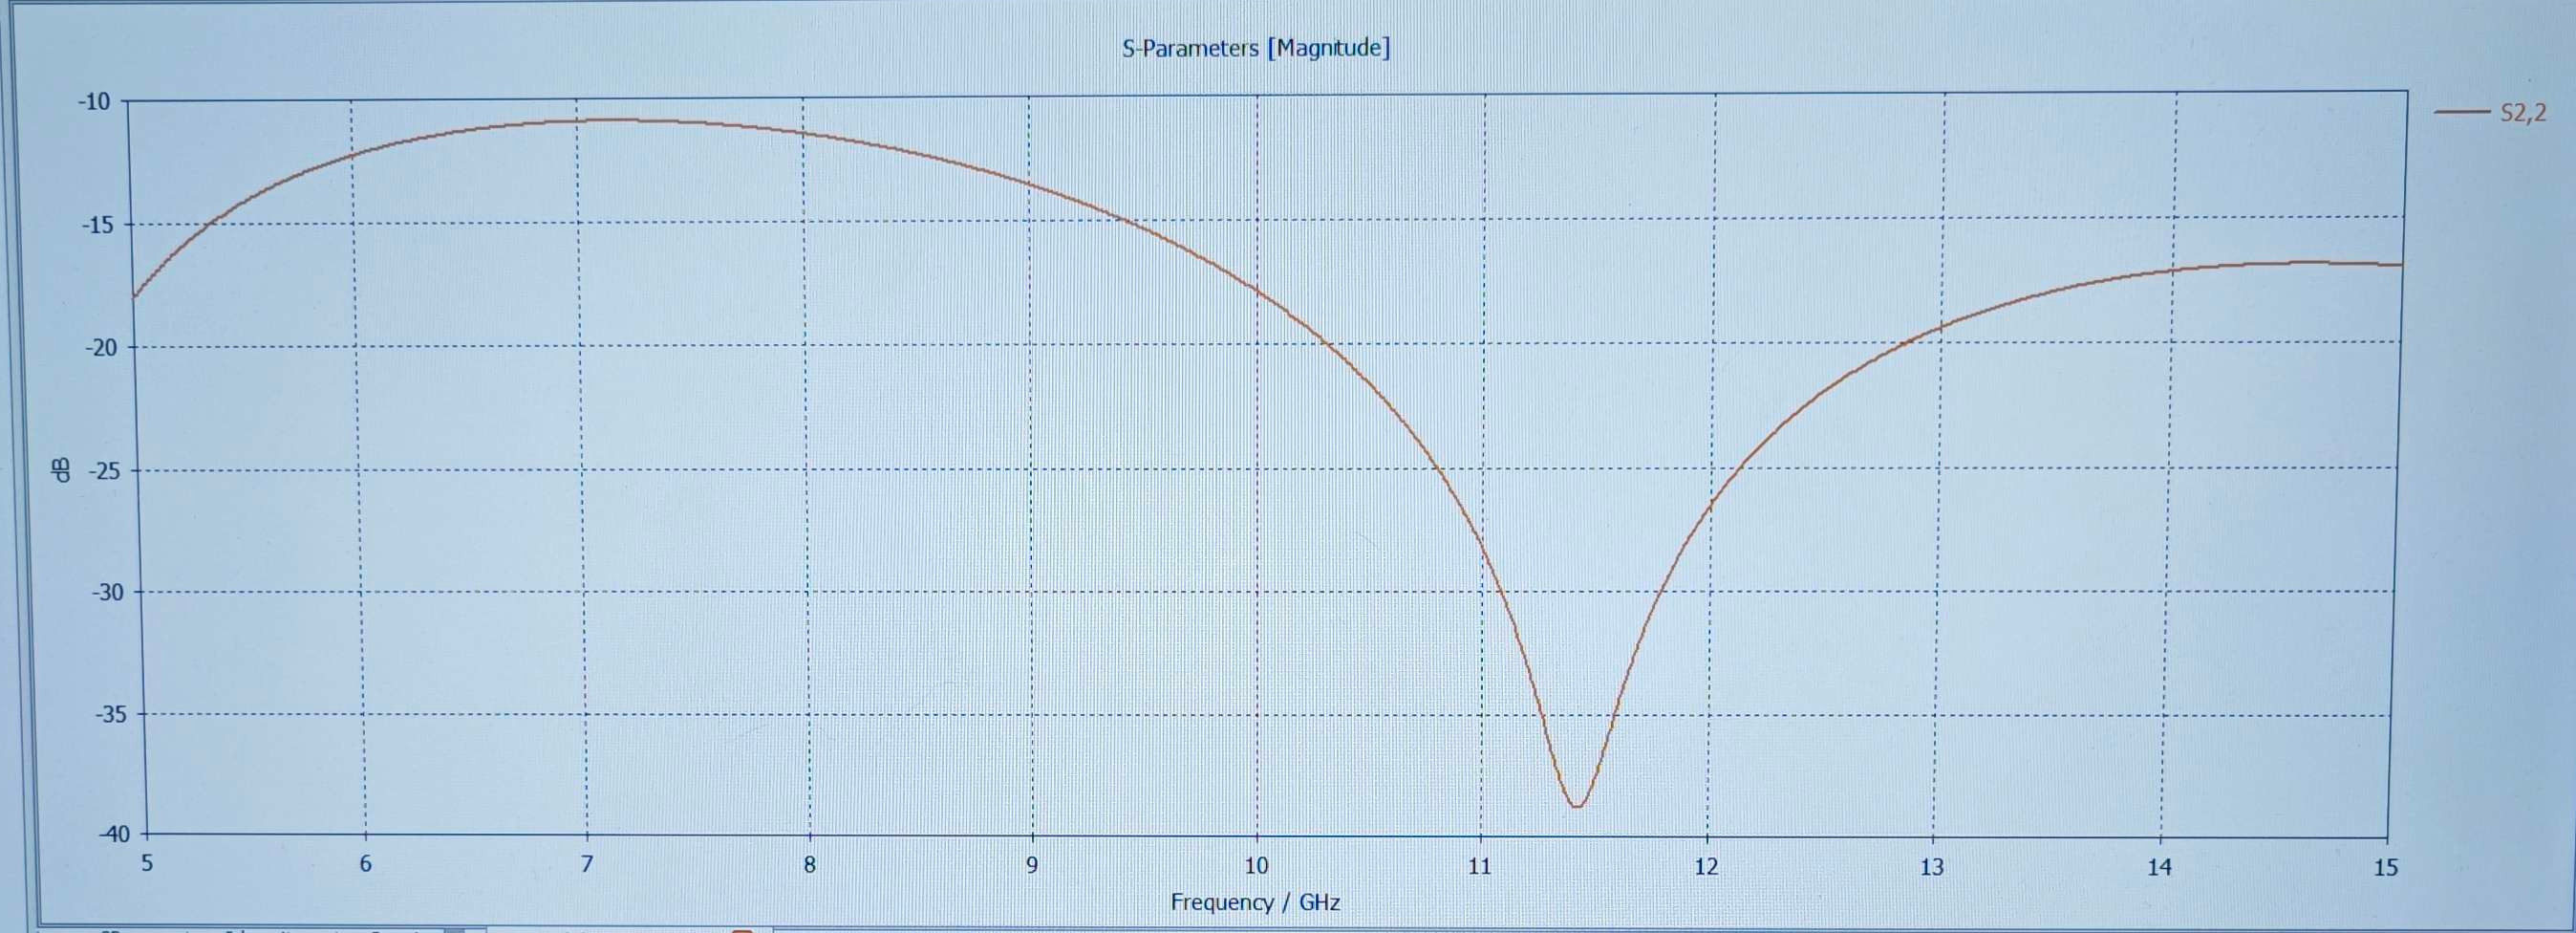
\includegraphics[width=.9\textwidth]{Figures/Lab Four/Line_S22.jpg}
  \caption{$S_{22}$ Parameter for the Transmission Line}
  \label{fig:4}
\end{figure}

\begin{figure}[H]
  \centering
  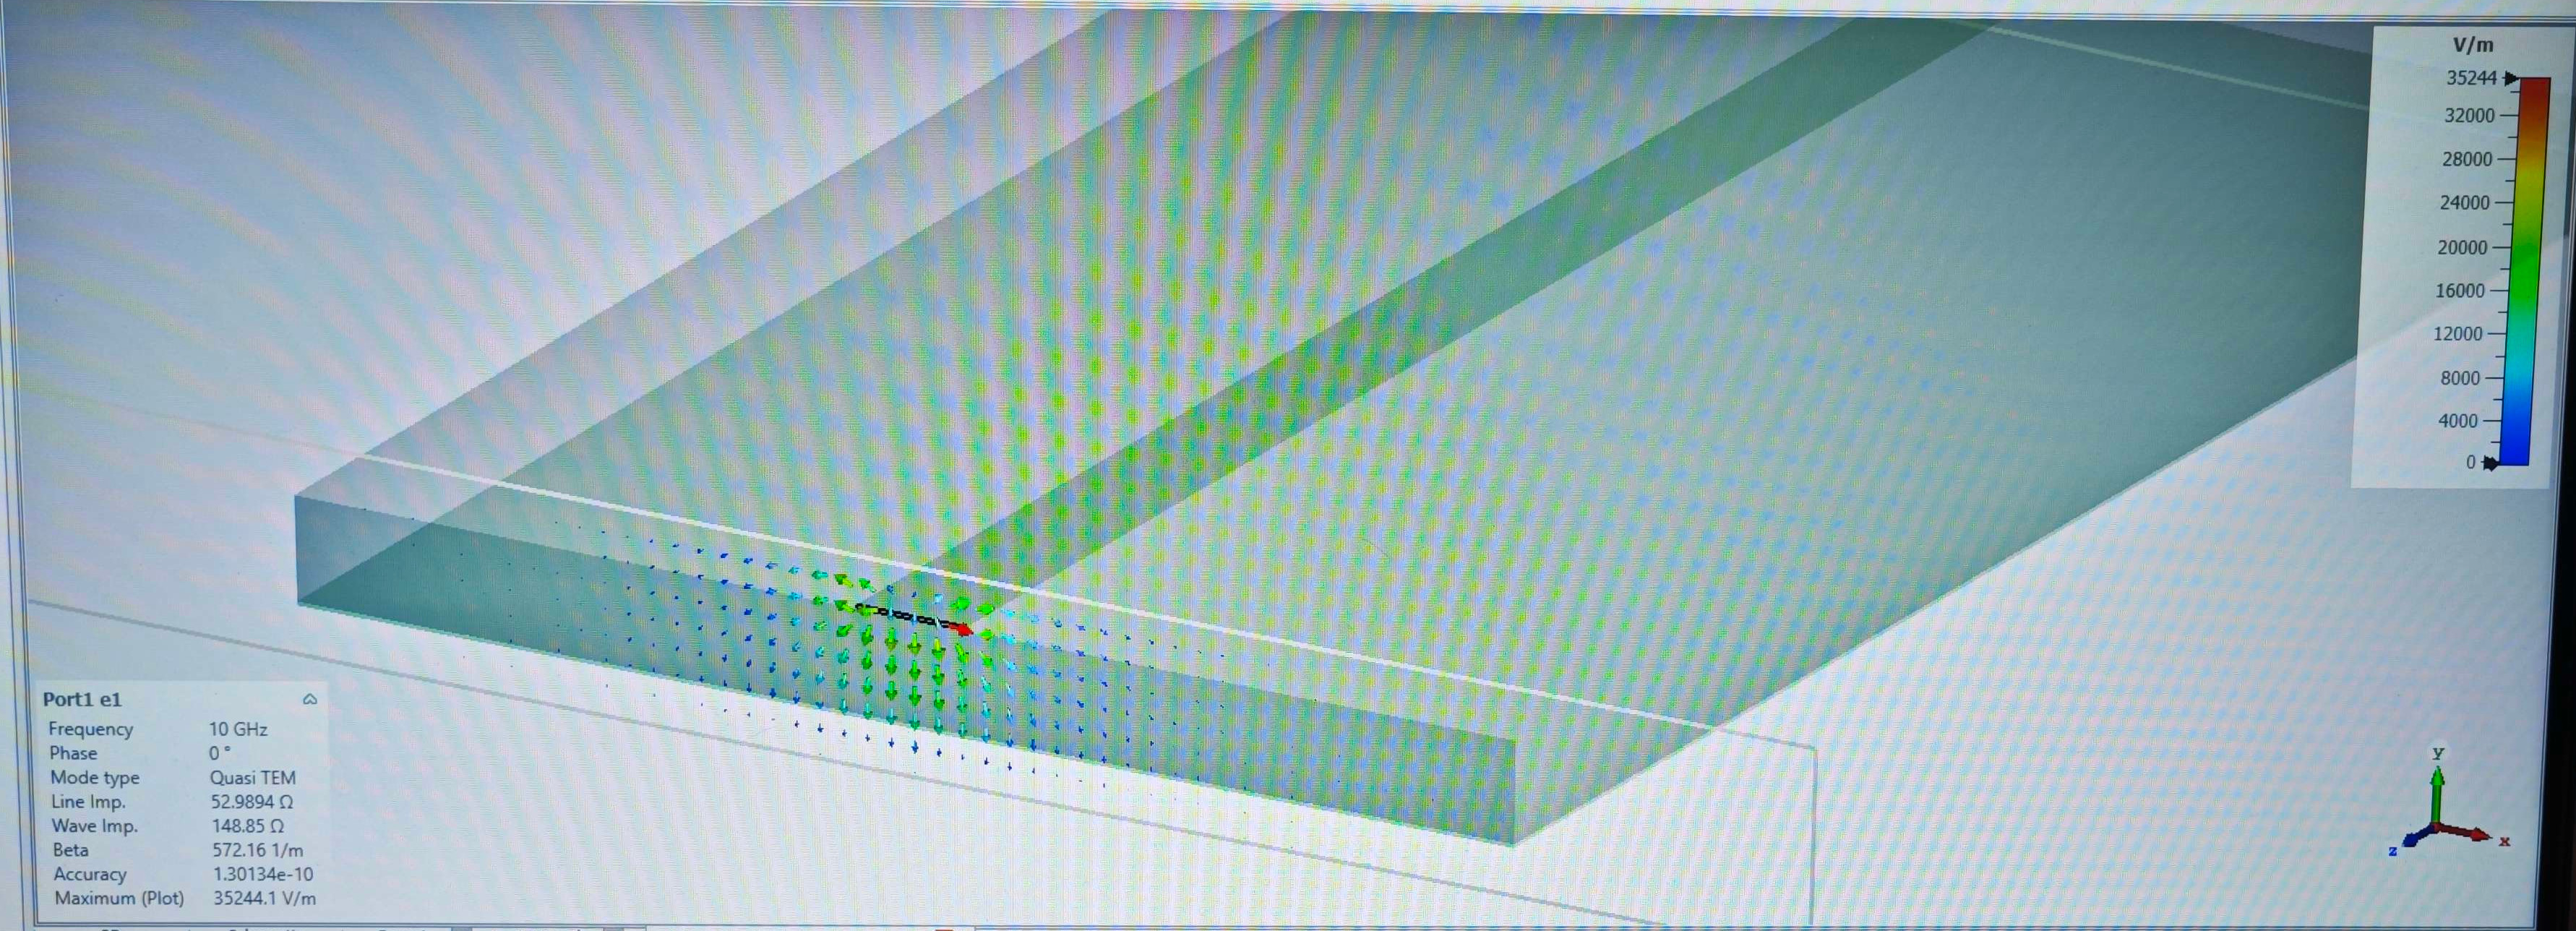
\includegraphics[width=.9\textwidth]{Figures/Lab Four/Front_EField.jpg}
  \caption{Unidimensional Electric Field from Front Port}
  \label{fig:5}
\end{figure}

\begin{figure}[H]
  \centering
  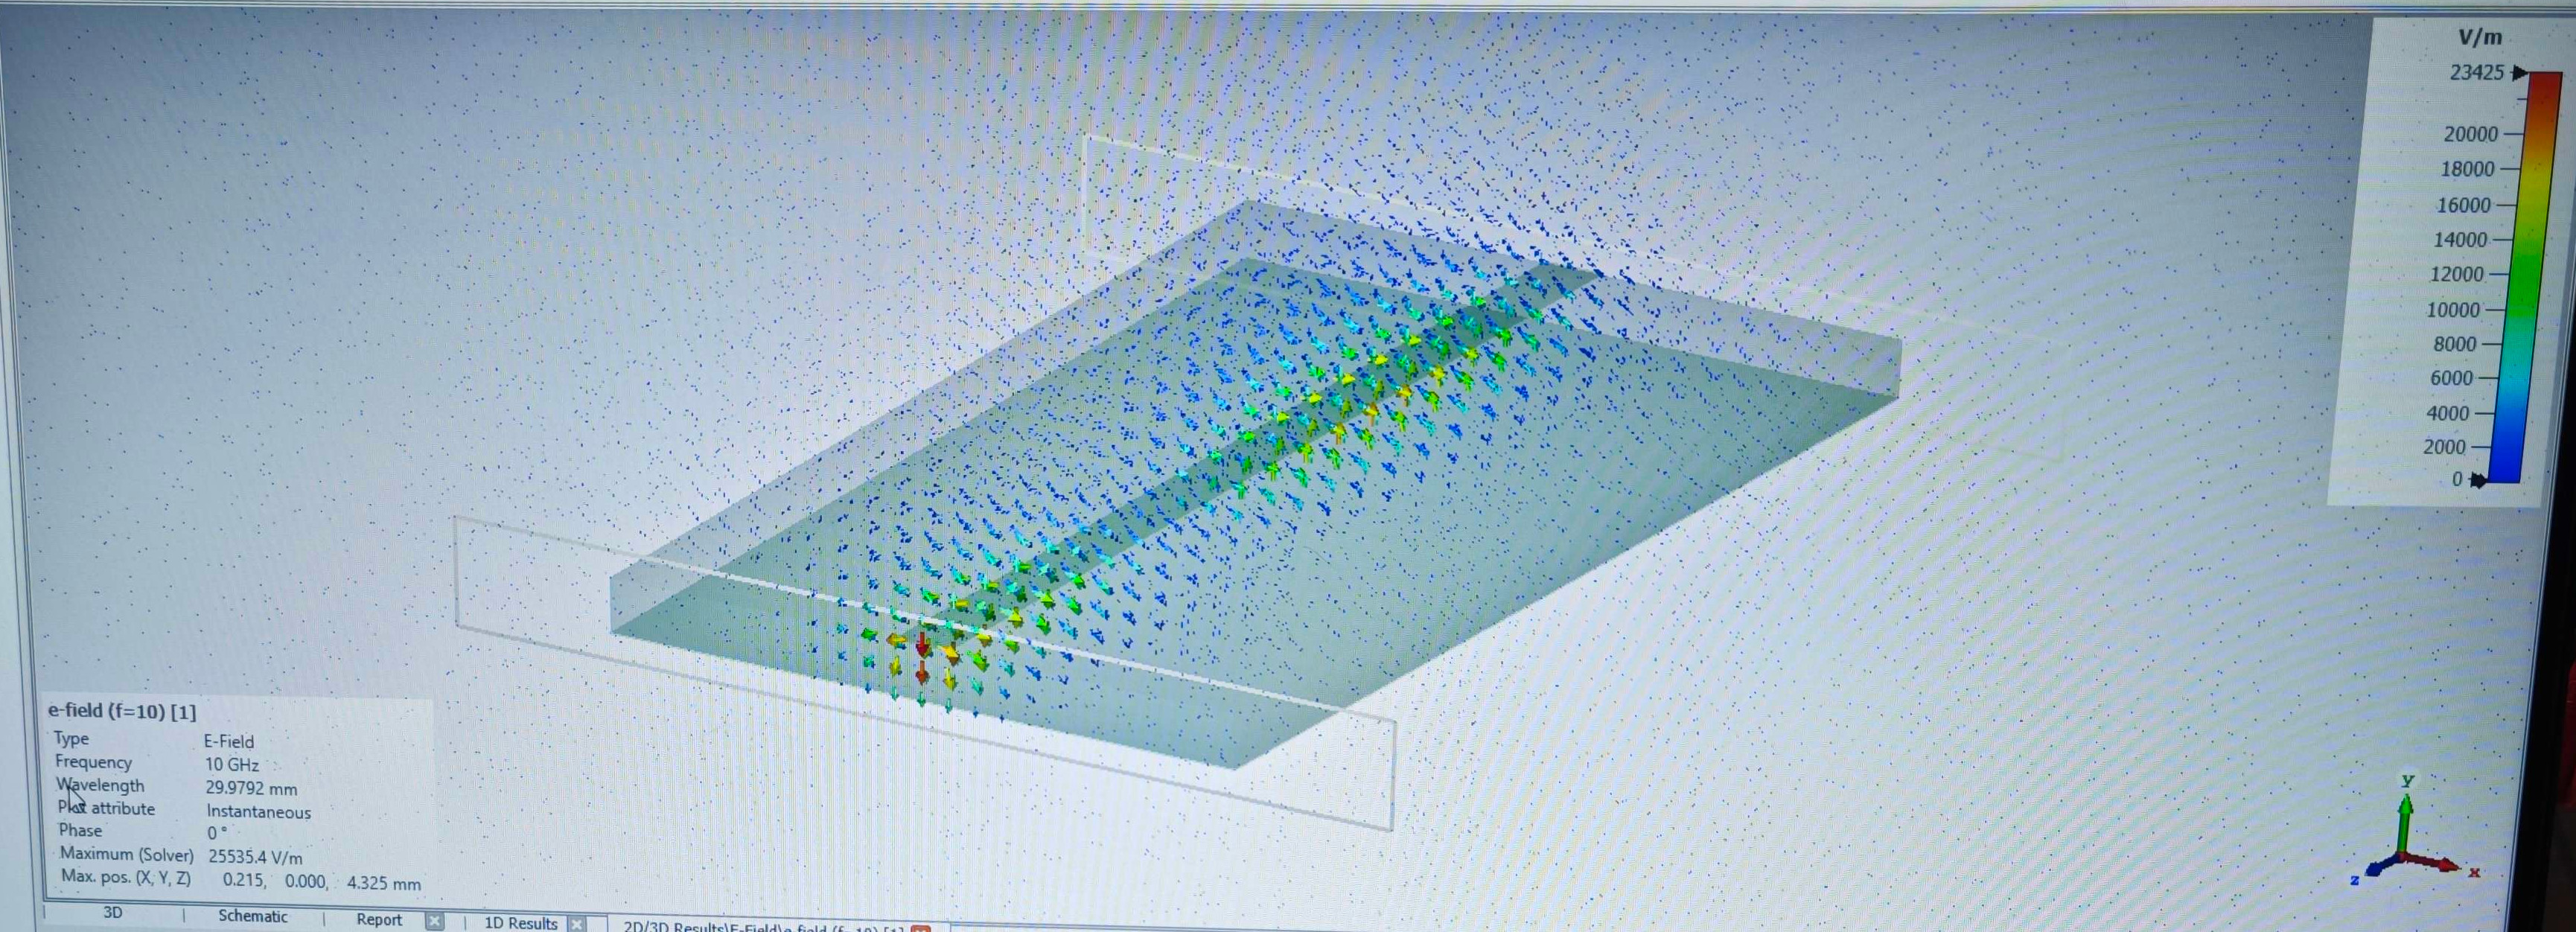
\includegraphics[width=.9\textwidth]{Figures/Lab Four/Front_EField_3D.jpg}
  \caption{Multidimensional Electric Field from Front Port}
  \label{fig:6}
\end{figure}

\begin{figure}[H]
  \centering
  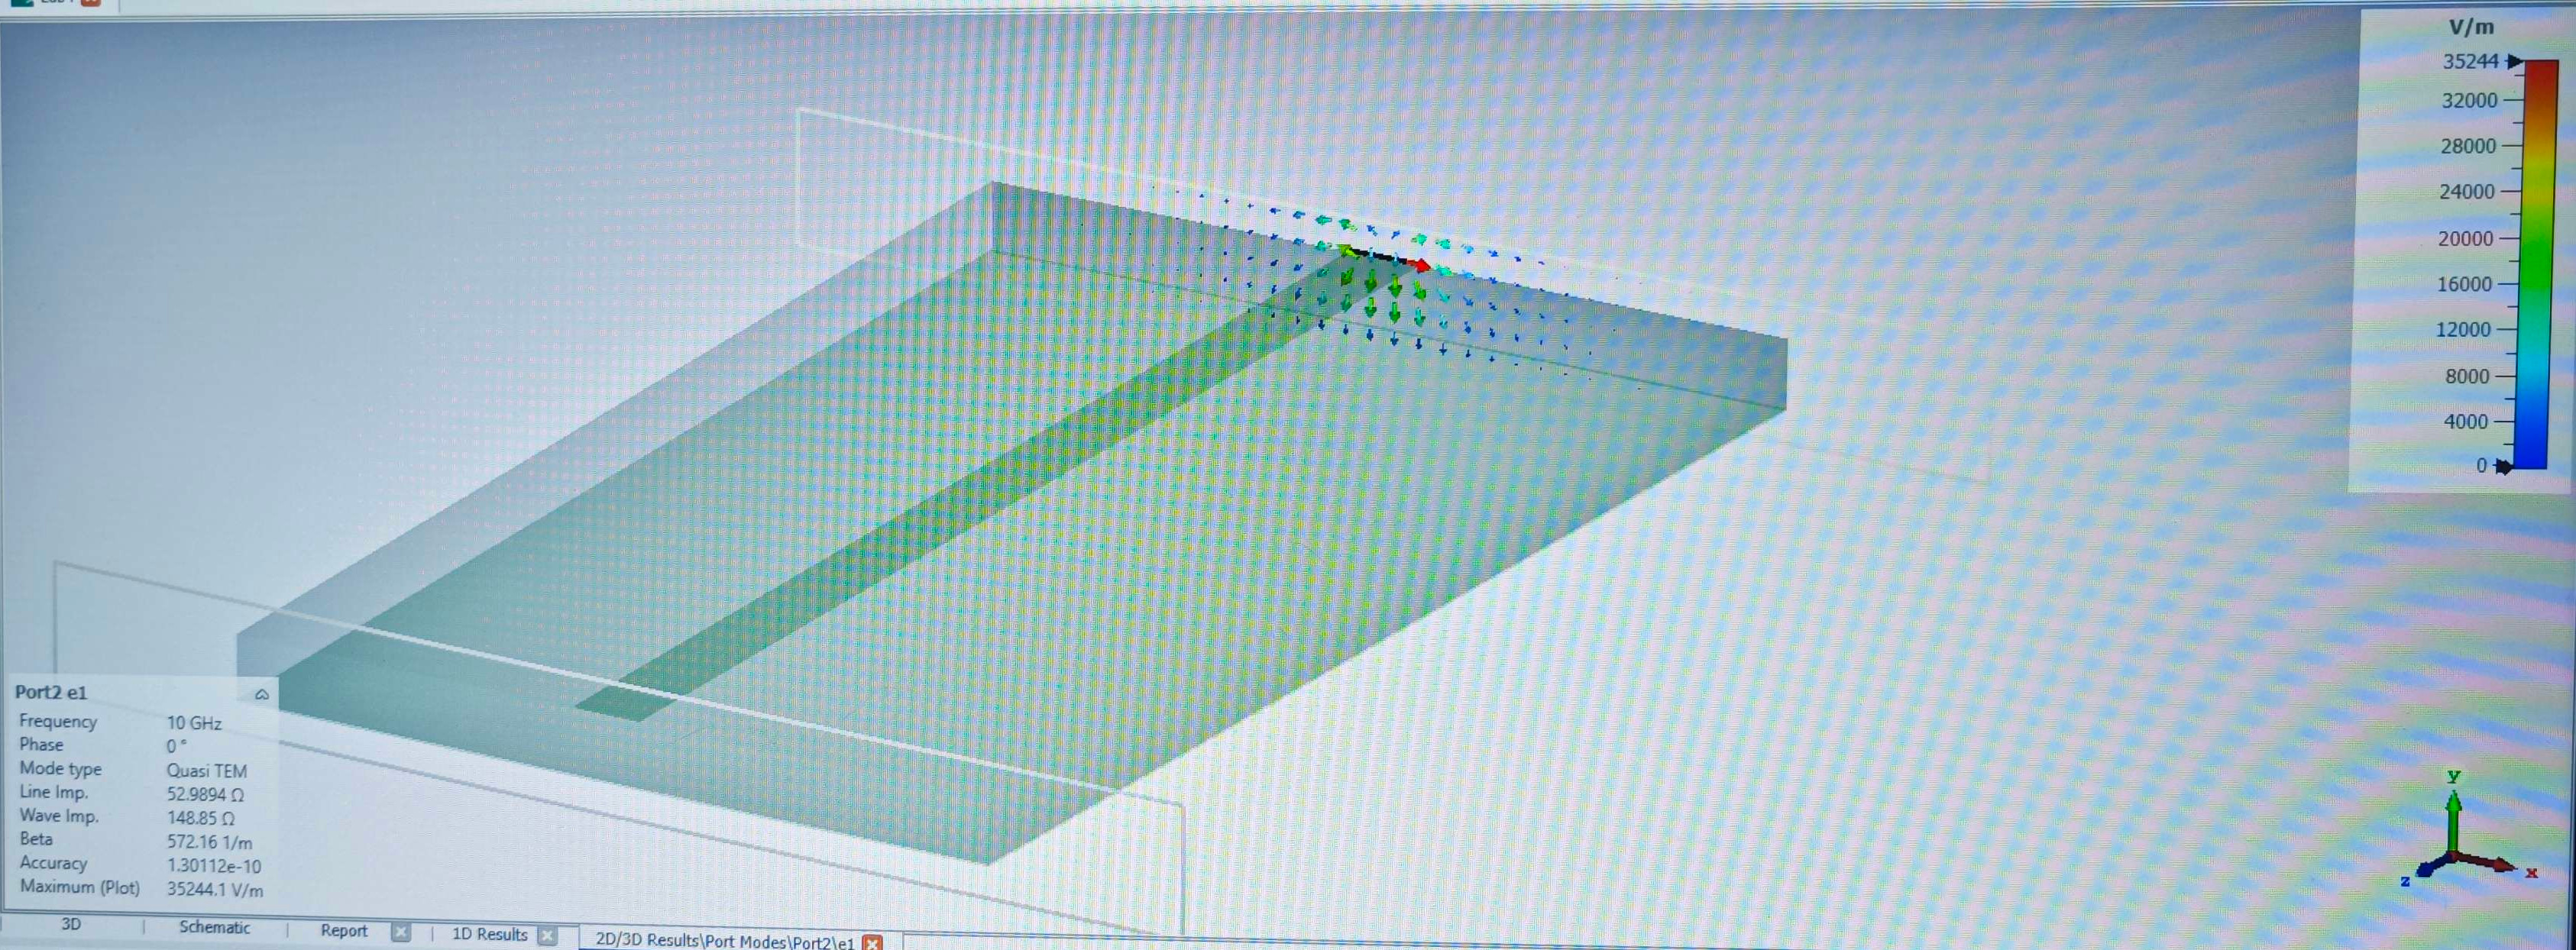
\includegraphics[width=.9\textwidth]{Figures/Lab Four/Rear_EField.jpg}
  \caption{Unidimensional Electric Field from Rear Port}
  \label{fig:7}
\end{figure}

\begin{figure}[H]
  \centering
  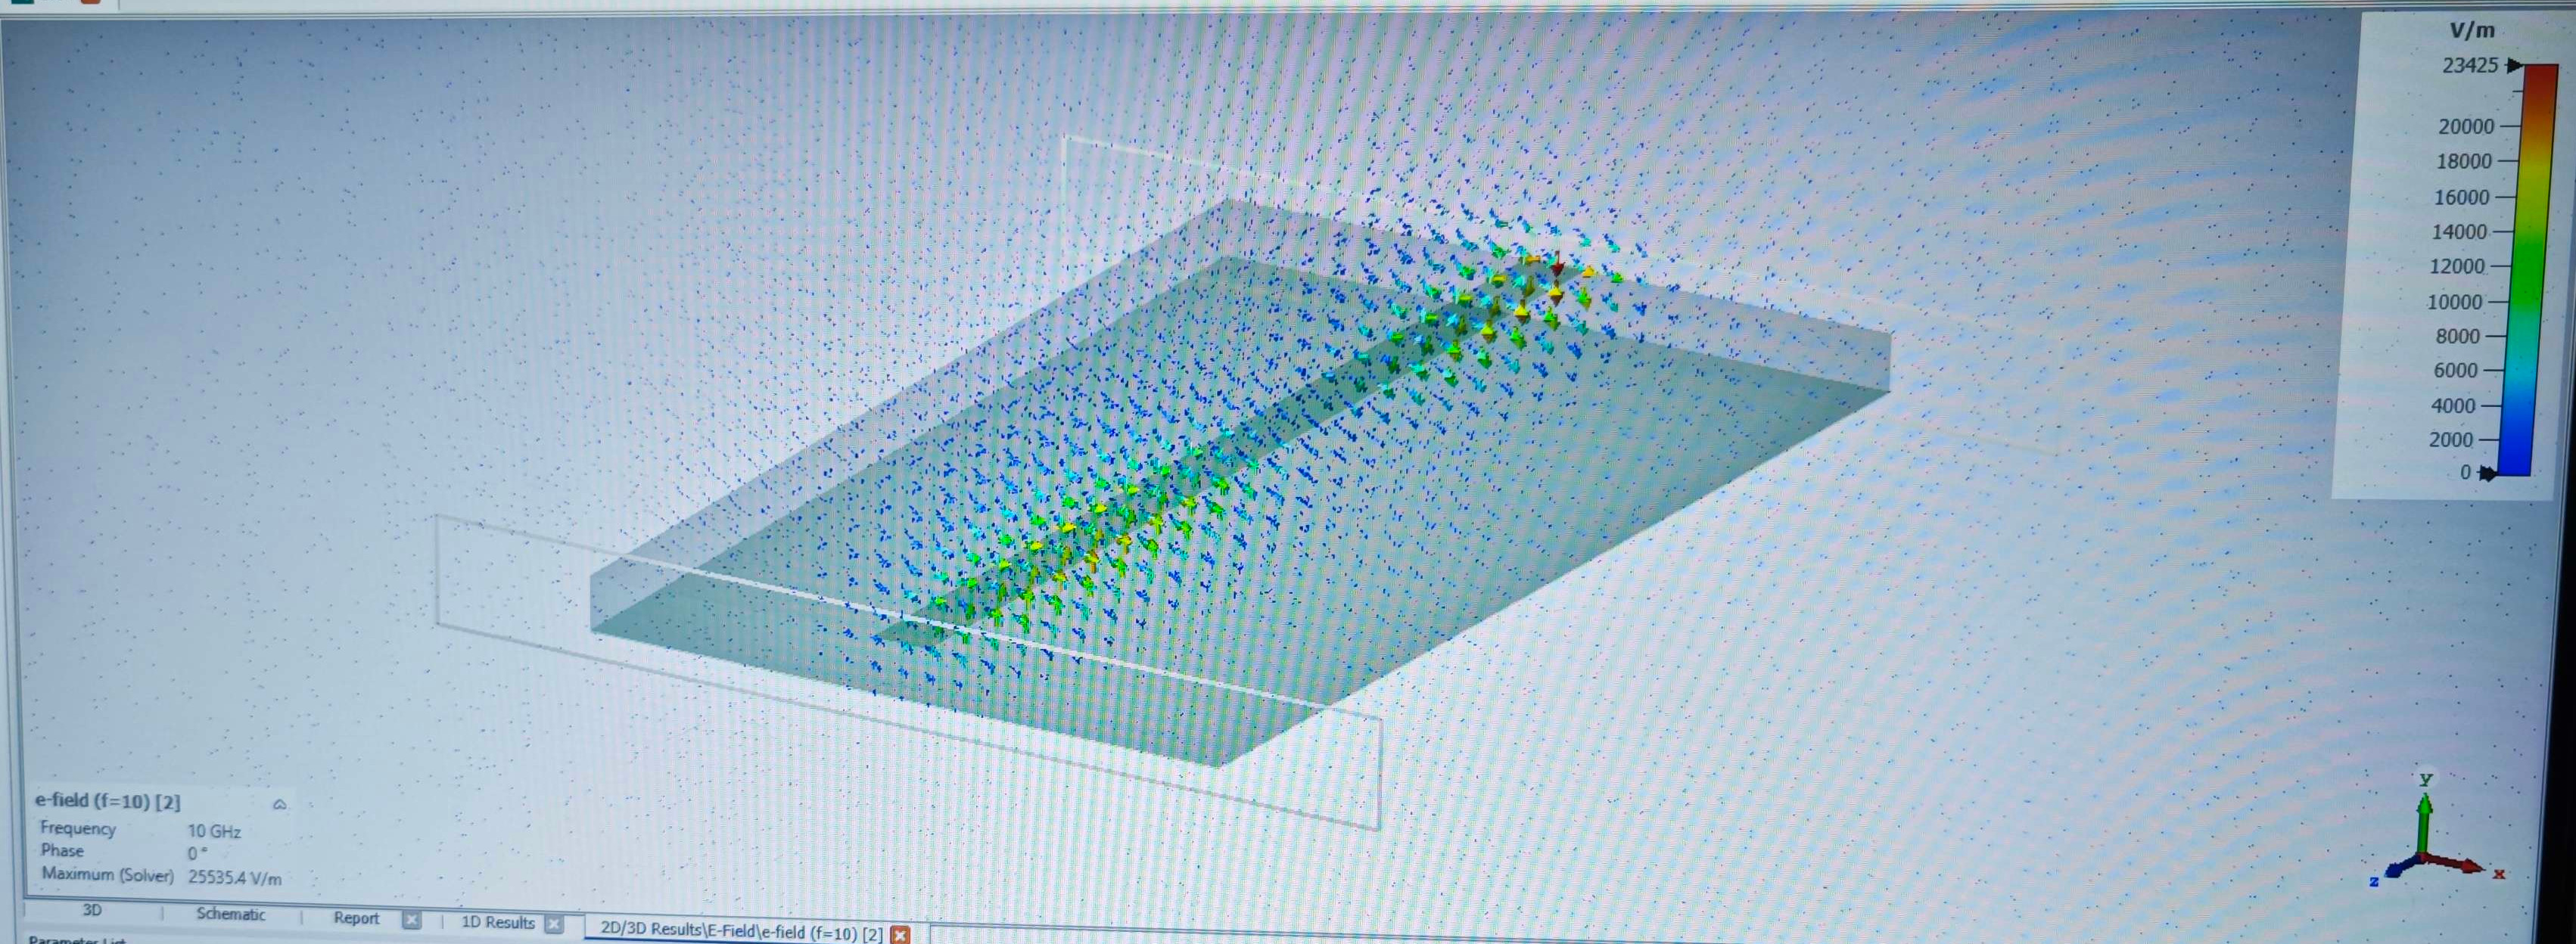
\includegraphics[width=.9\textwidth]{Figures/Lab Four/Rear_EField_3D.jpg}
  \caption{Multidimensional Electric Field from Rear Port}
  \label{fig:8}
\end{figure}

\begin{figure}[H]
  \centering
  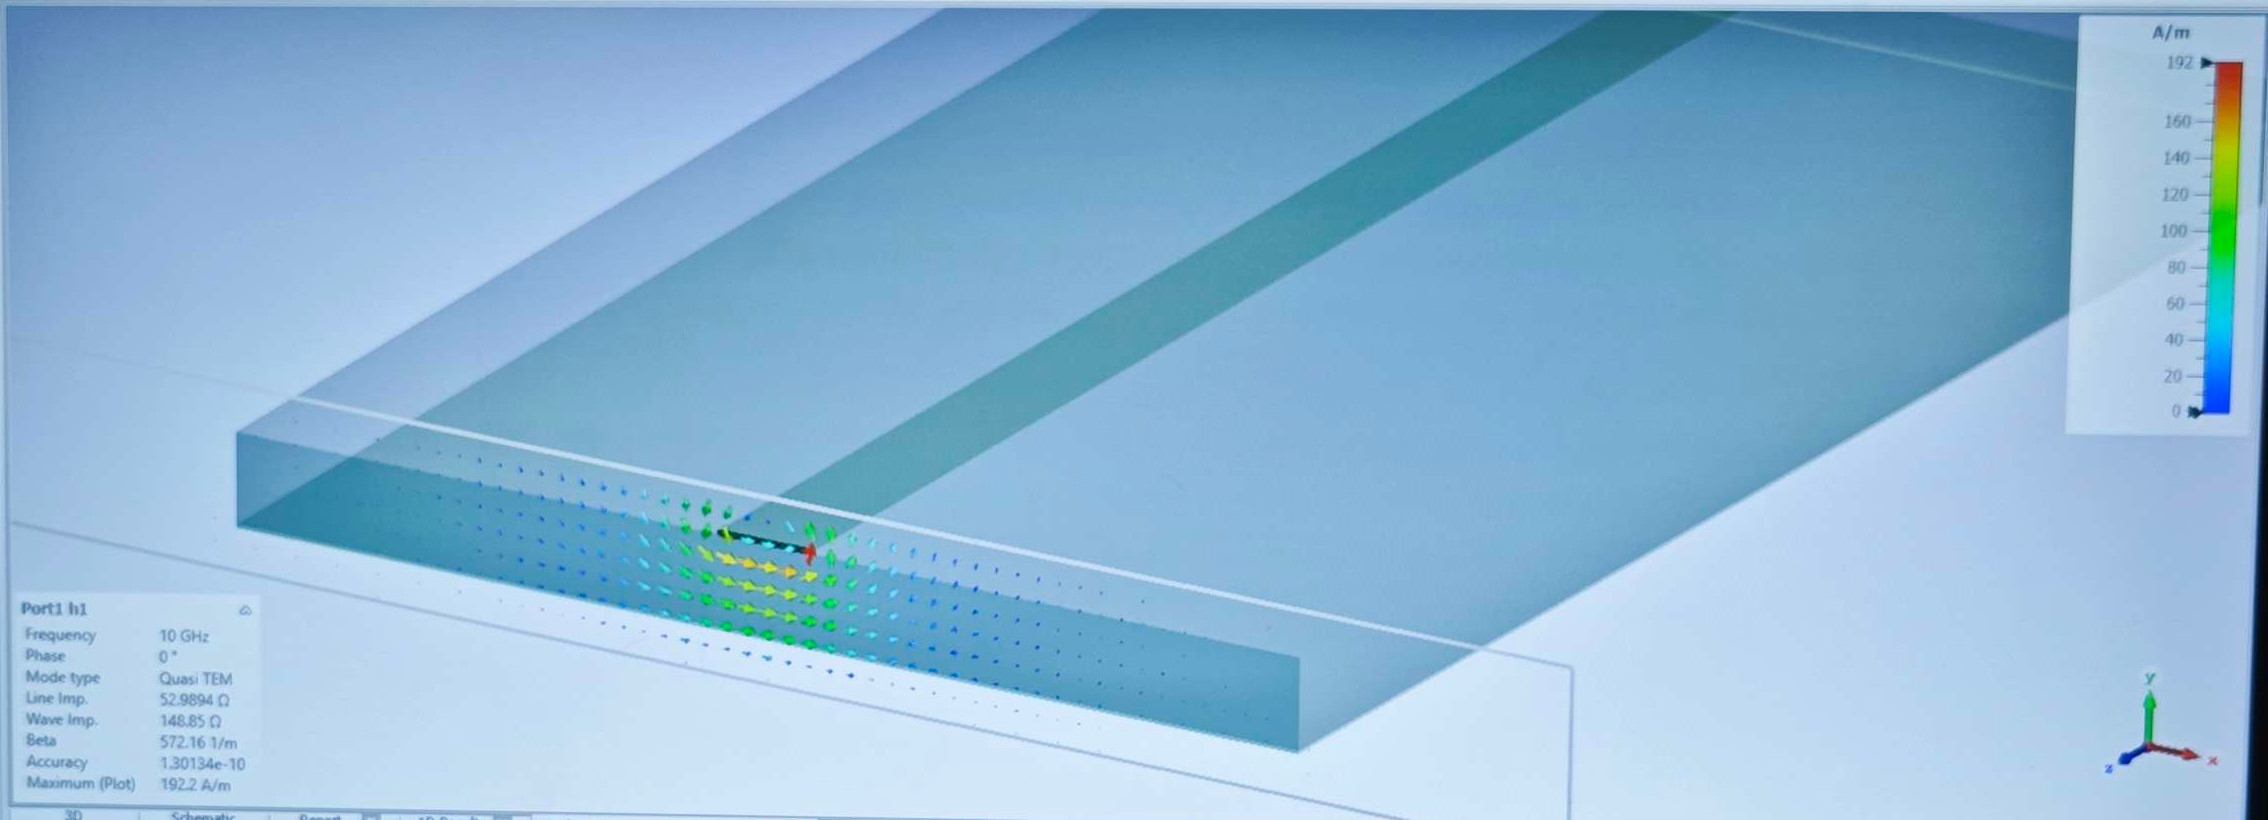
\includegraphics[width=.9\textwidth]{Figures/Lab Four/Front_BField.jpg}
  \caption{Unidimensional Magnetic Field from Front Port}
  \label{fig:9}
\end{figure}

\begin{figure}[H]
  \centering
  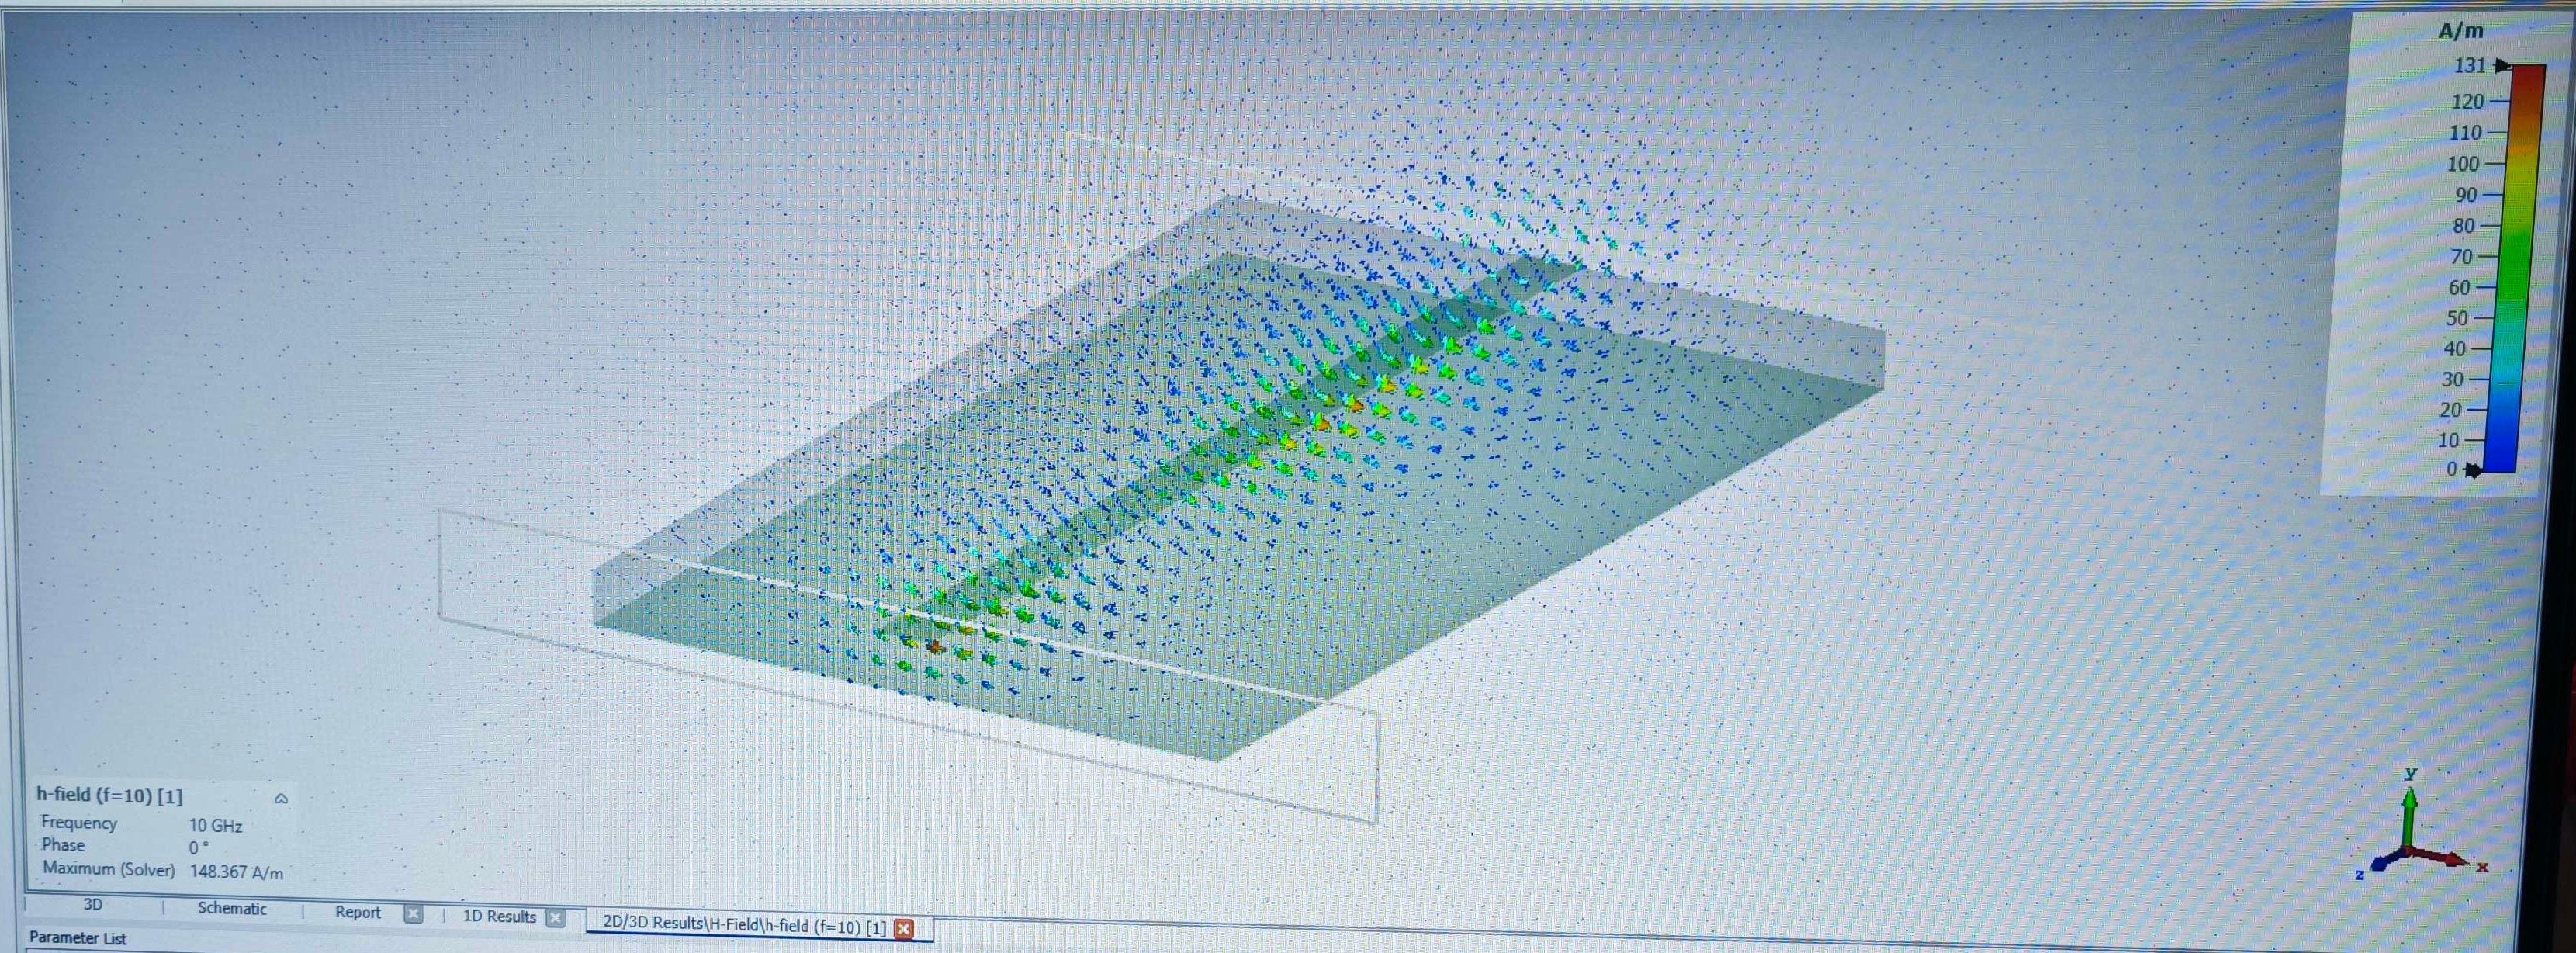
\includegraphics[width=.9\textwidth]{Figures/Lab Four/Front_BField_3D.jpg}
  \caption{Multidimensional Magnetic Field from Front Port}
  \label{fig:10}
\end{figure}

\begin{figure}[H]
  \centering
  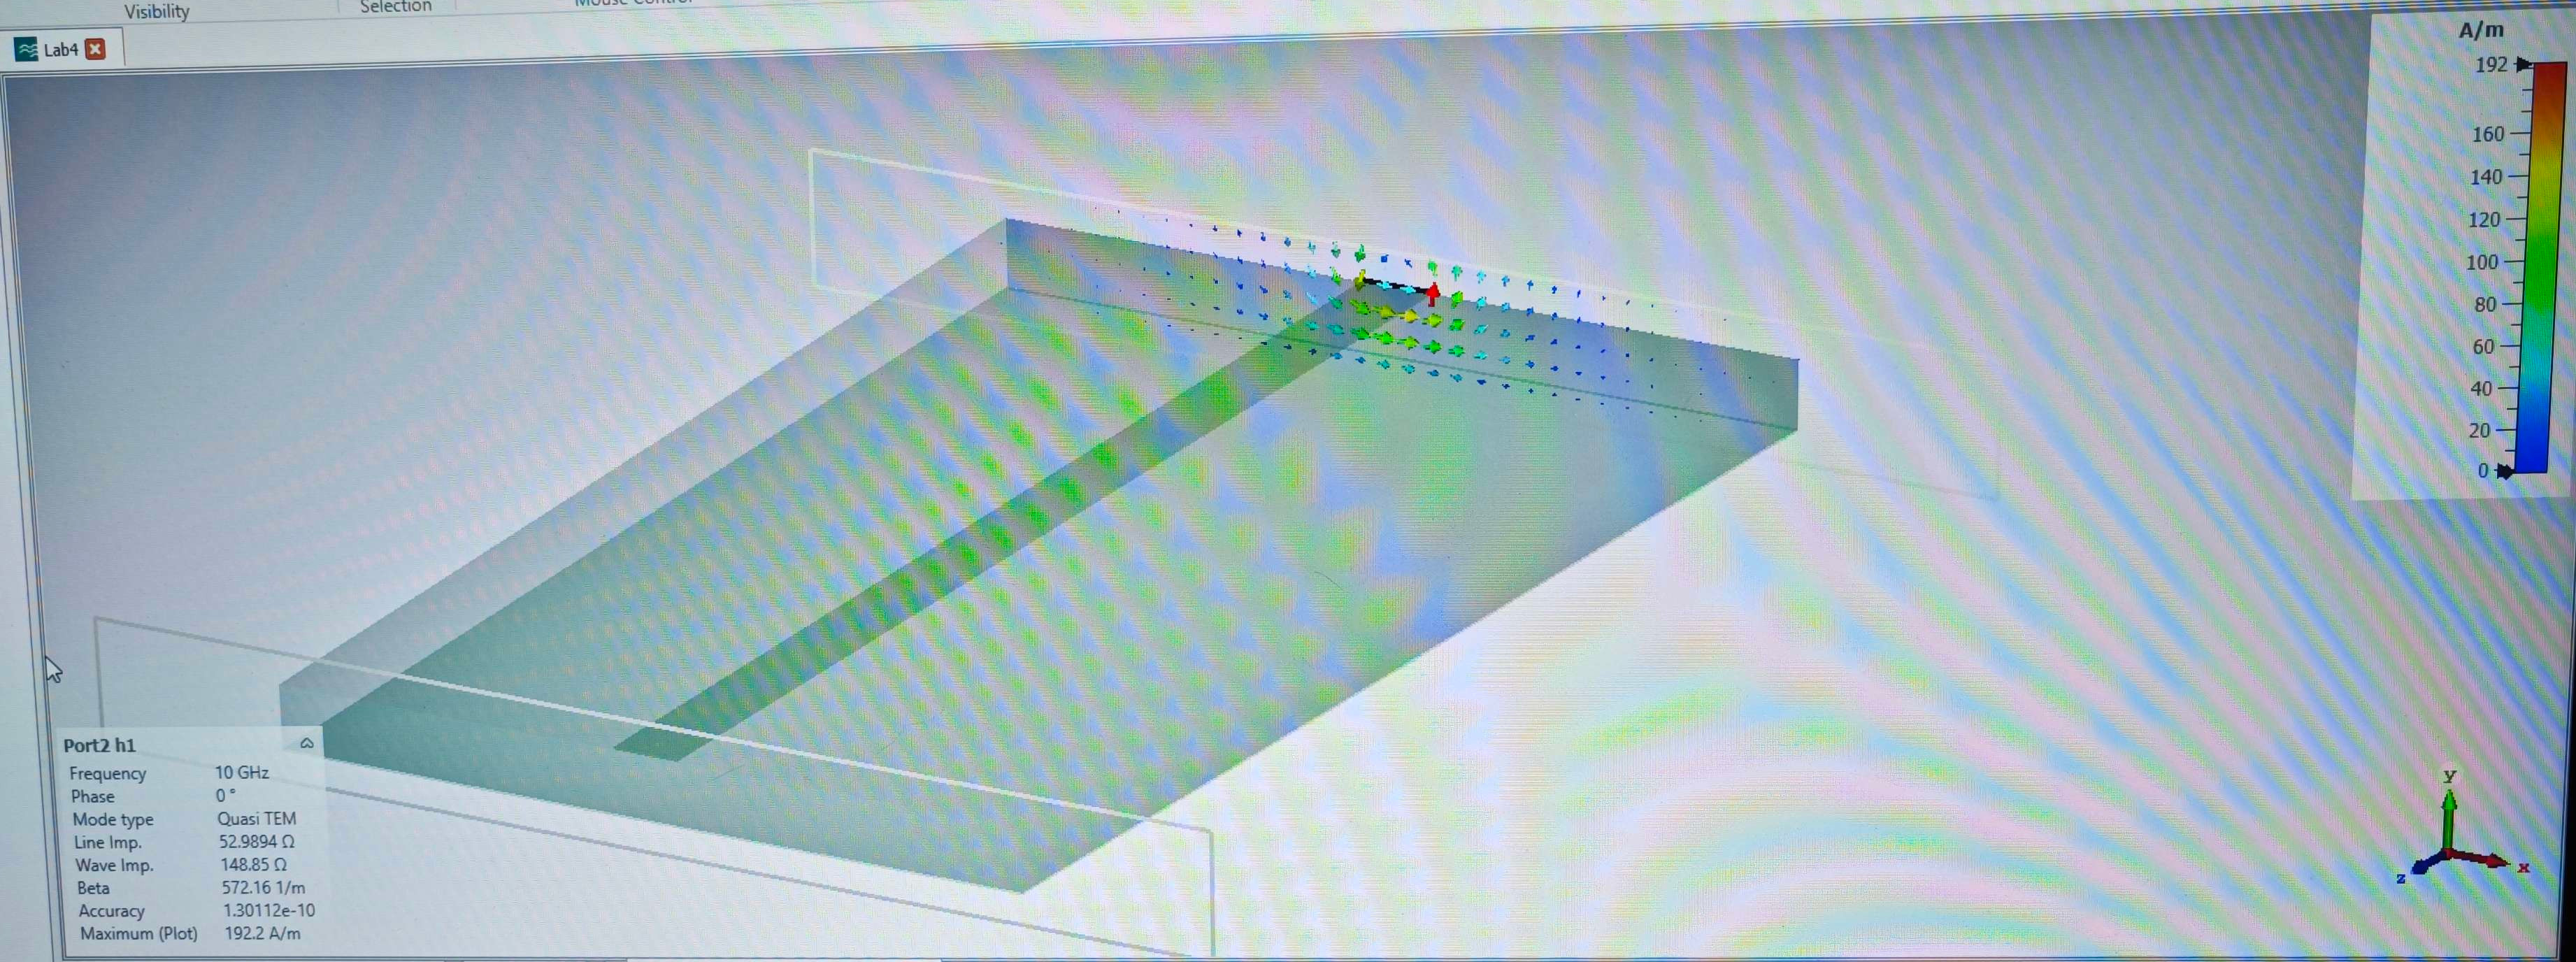
\includegraphics[width=.9\textwidth]{Figures/Lab Four/Rear_BField.jpg}
  \caption{Unidimensional Magnetic Field from Rear Port}
  \label{fig:11}
\end{figure}

\begin{figure}[H]
  \centering
  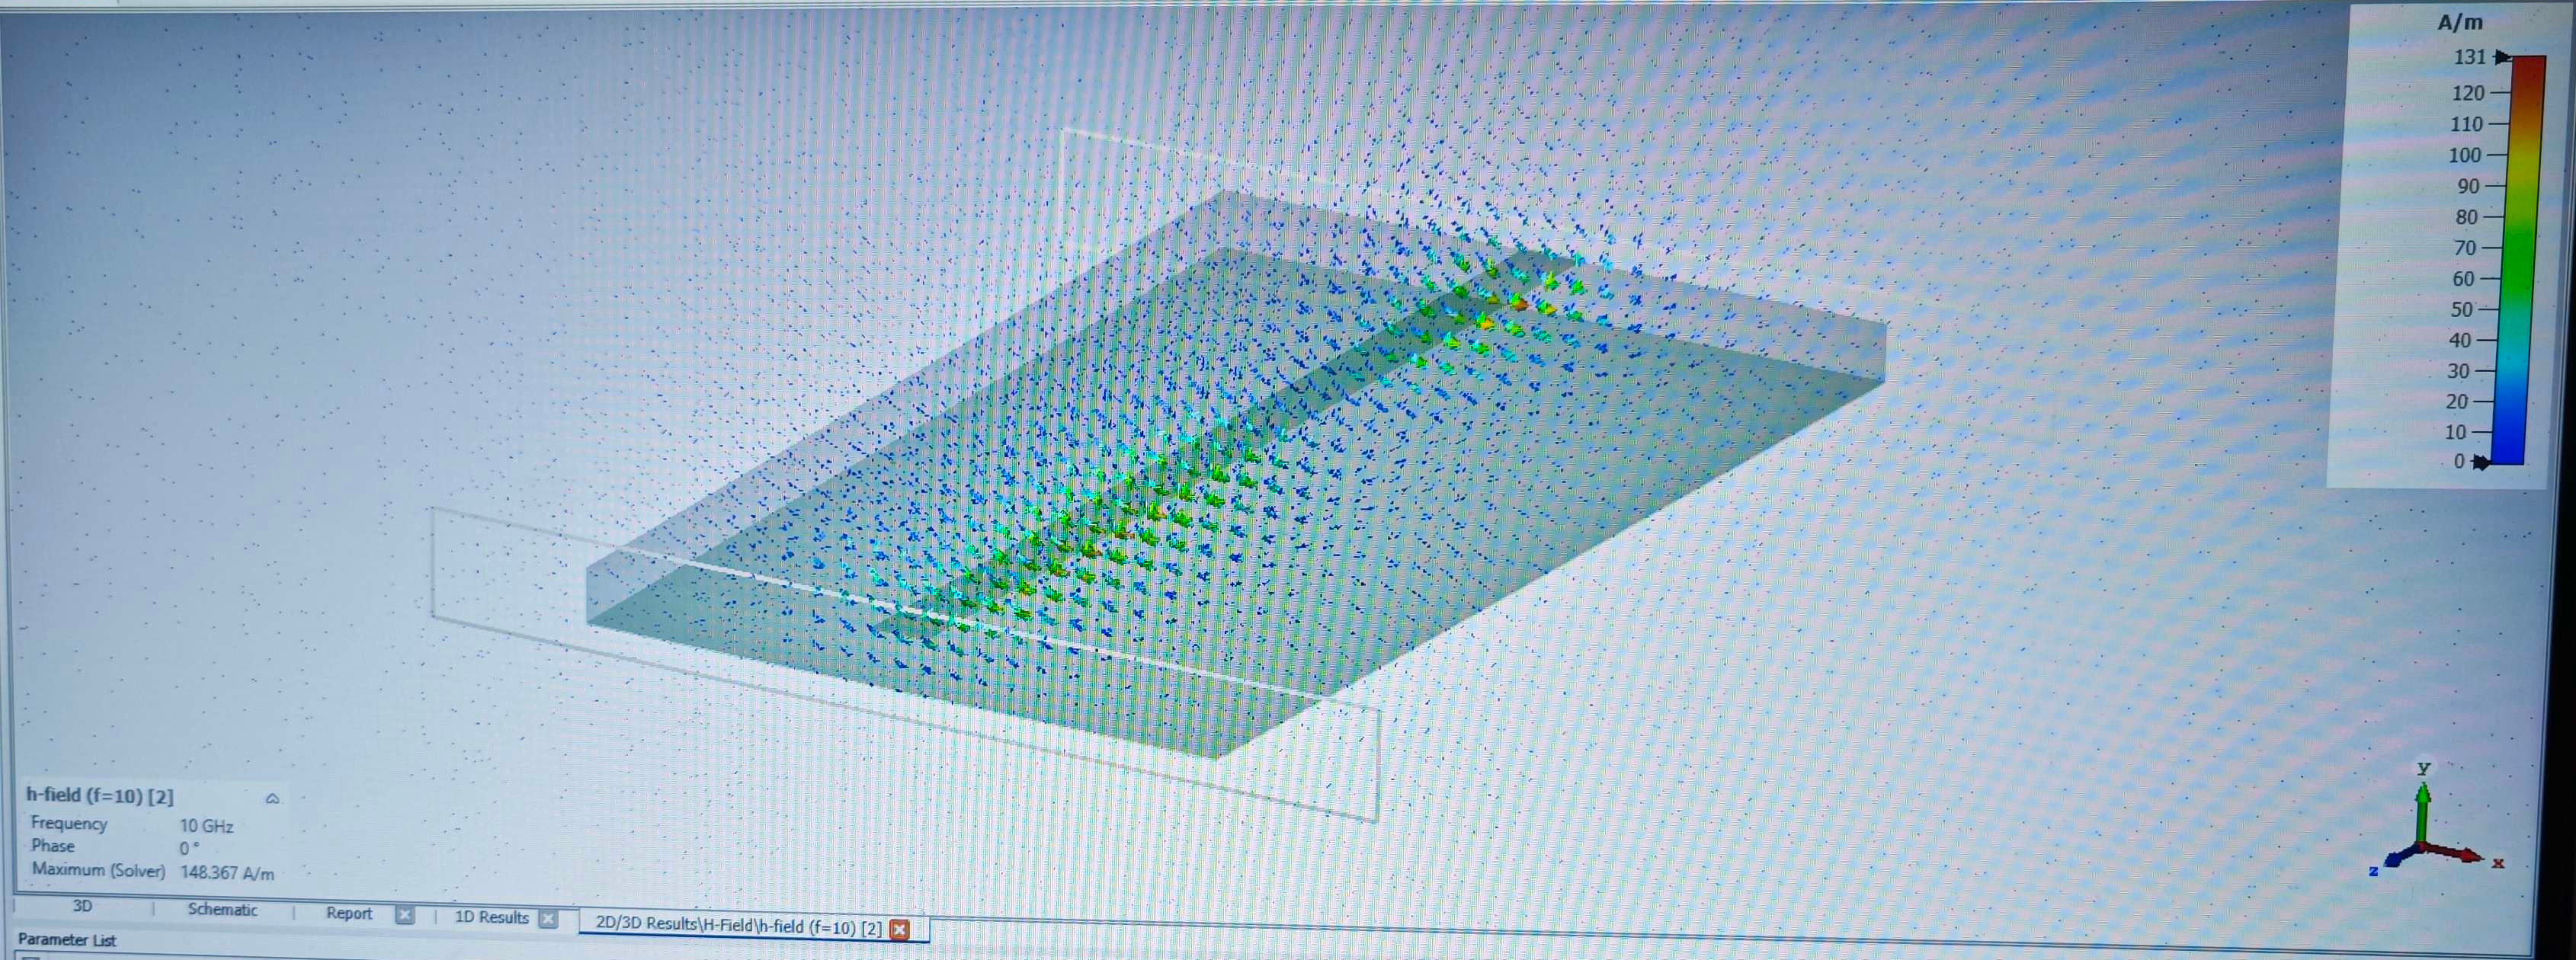
\includegraphics[width=.9\textwidth]{Figures/Lab Four/Rear_BField_3D.jpg}
  \caption{Multidimensional Magnetic Field from Rear Port}
  \label{fig:12}
\end{figure}

For the resonator strip, simulations were run to generate $S$ parameter graphs, which can be seen in Figures \ref{fig:13}-\ref{fig:17} below:

\begin{figure}[H]
  \centering
  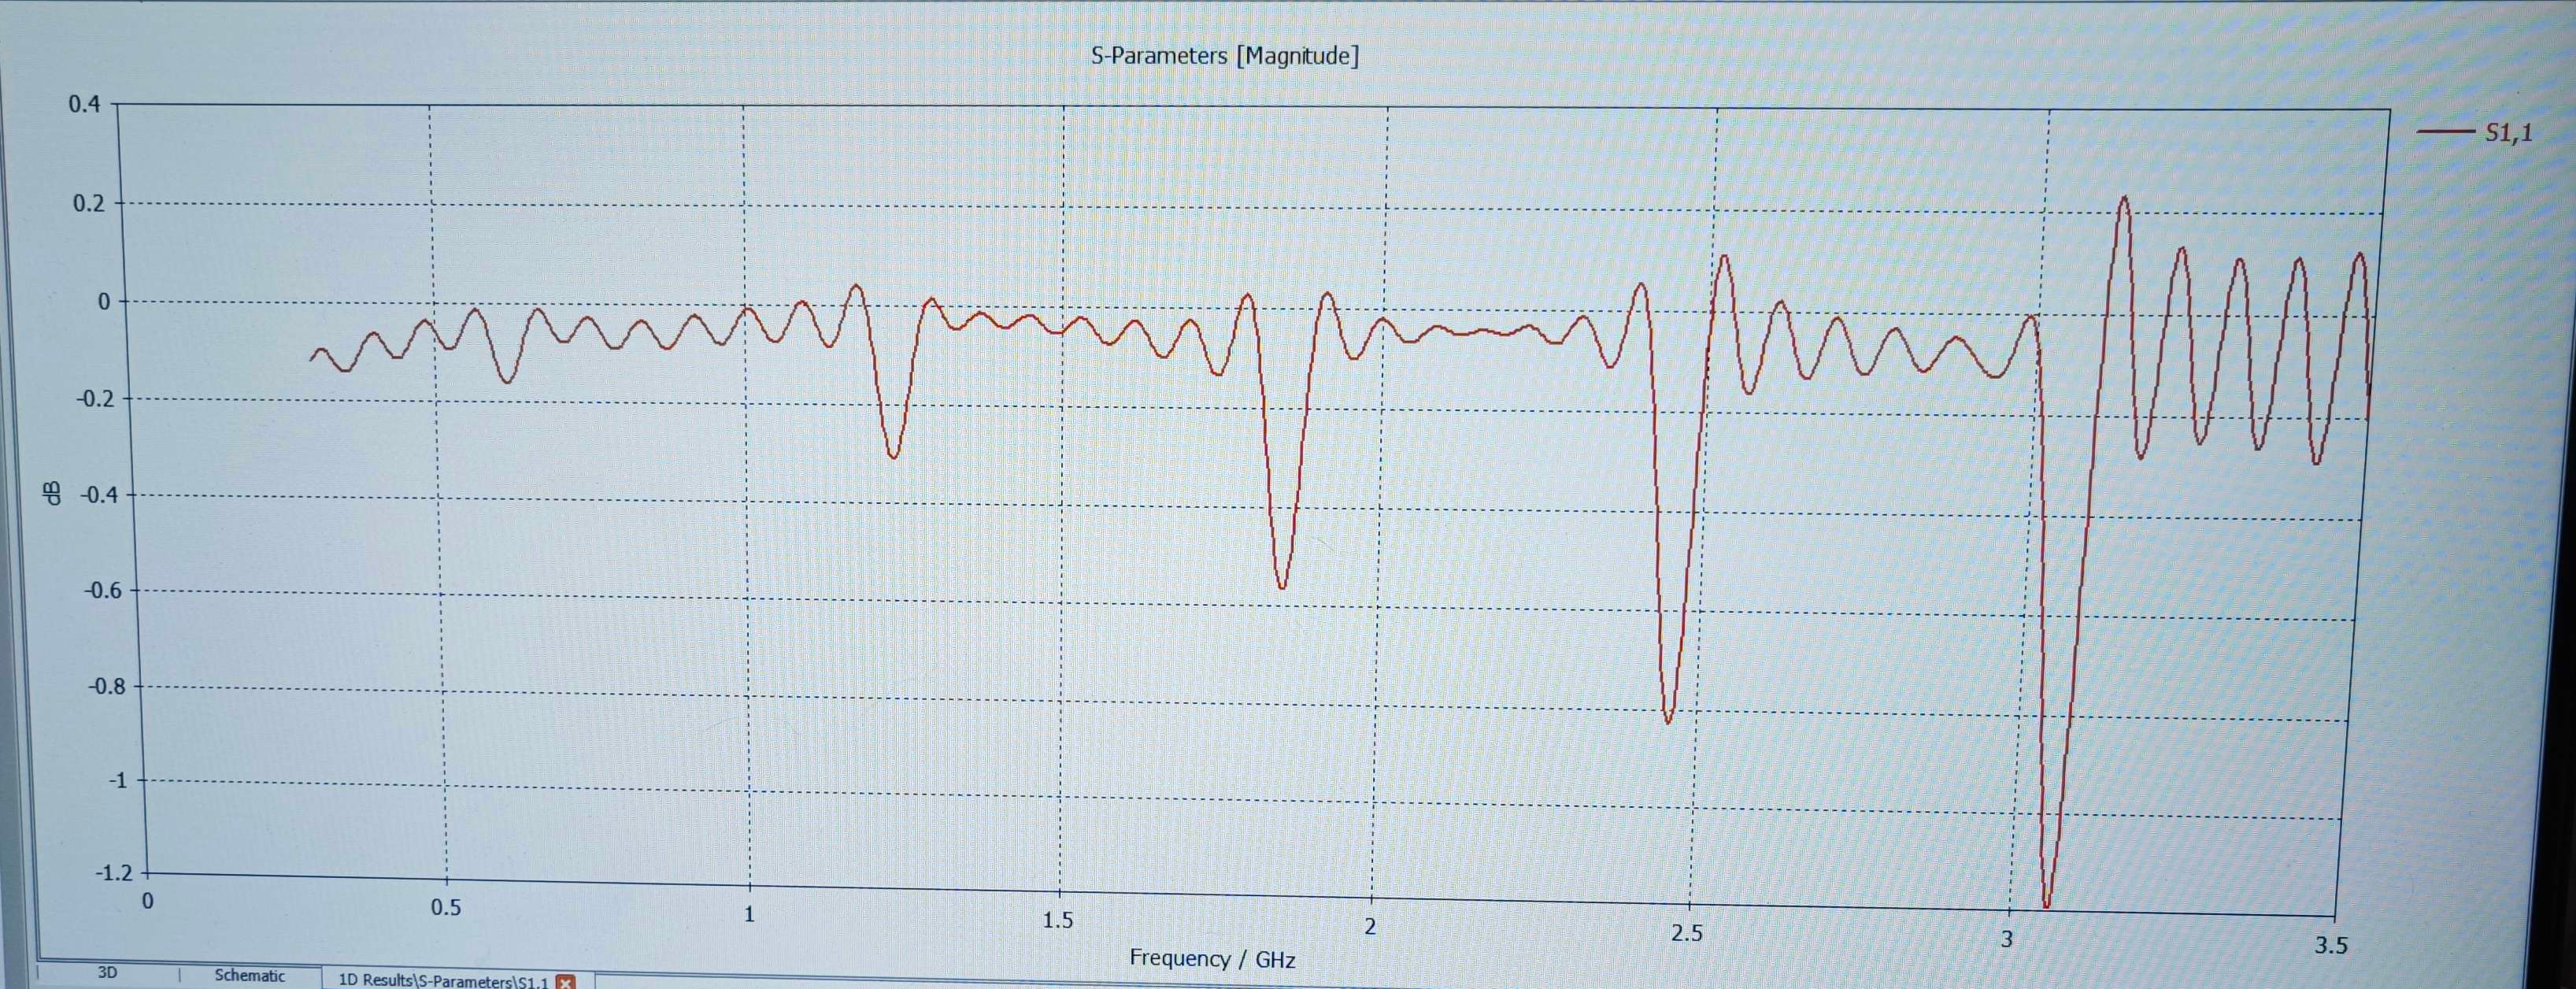
\includegraphics[width=.9\textwidth]{Figures/Lab Four/Resonator_S11.jpg}
  \caption{Resonator $S_{11}$ Plot}
  \label{fig:13}
\end{figure}

\begin{figure}[H]
  \centering
  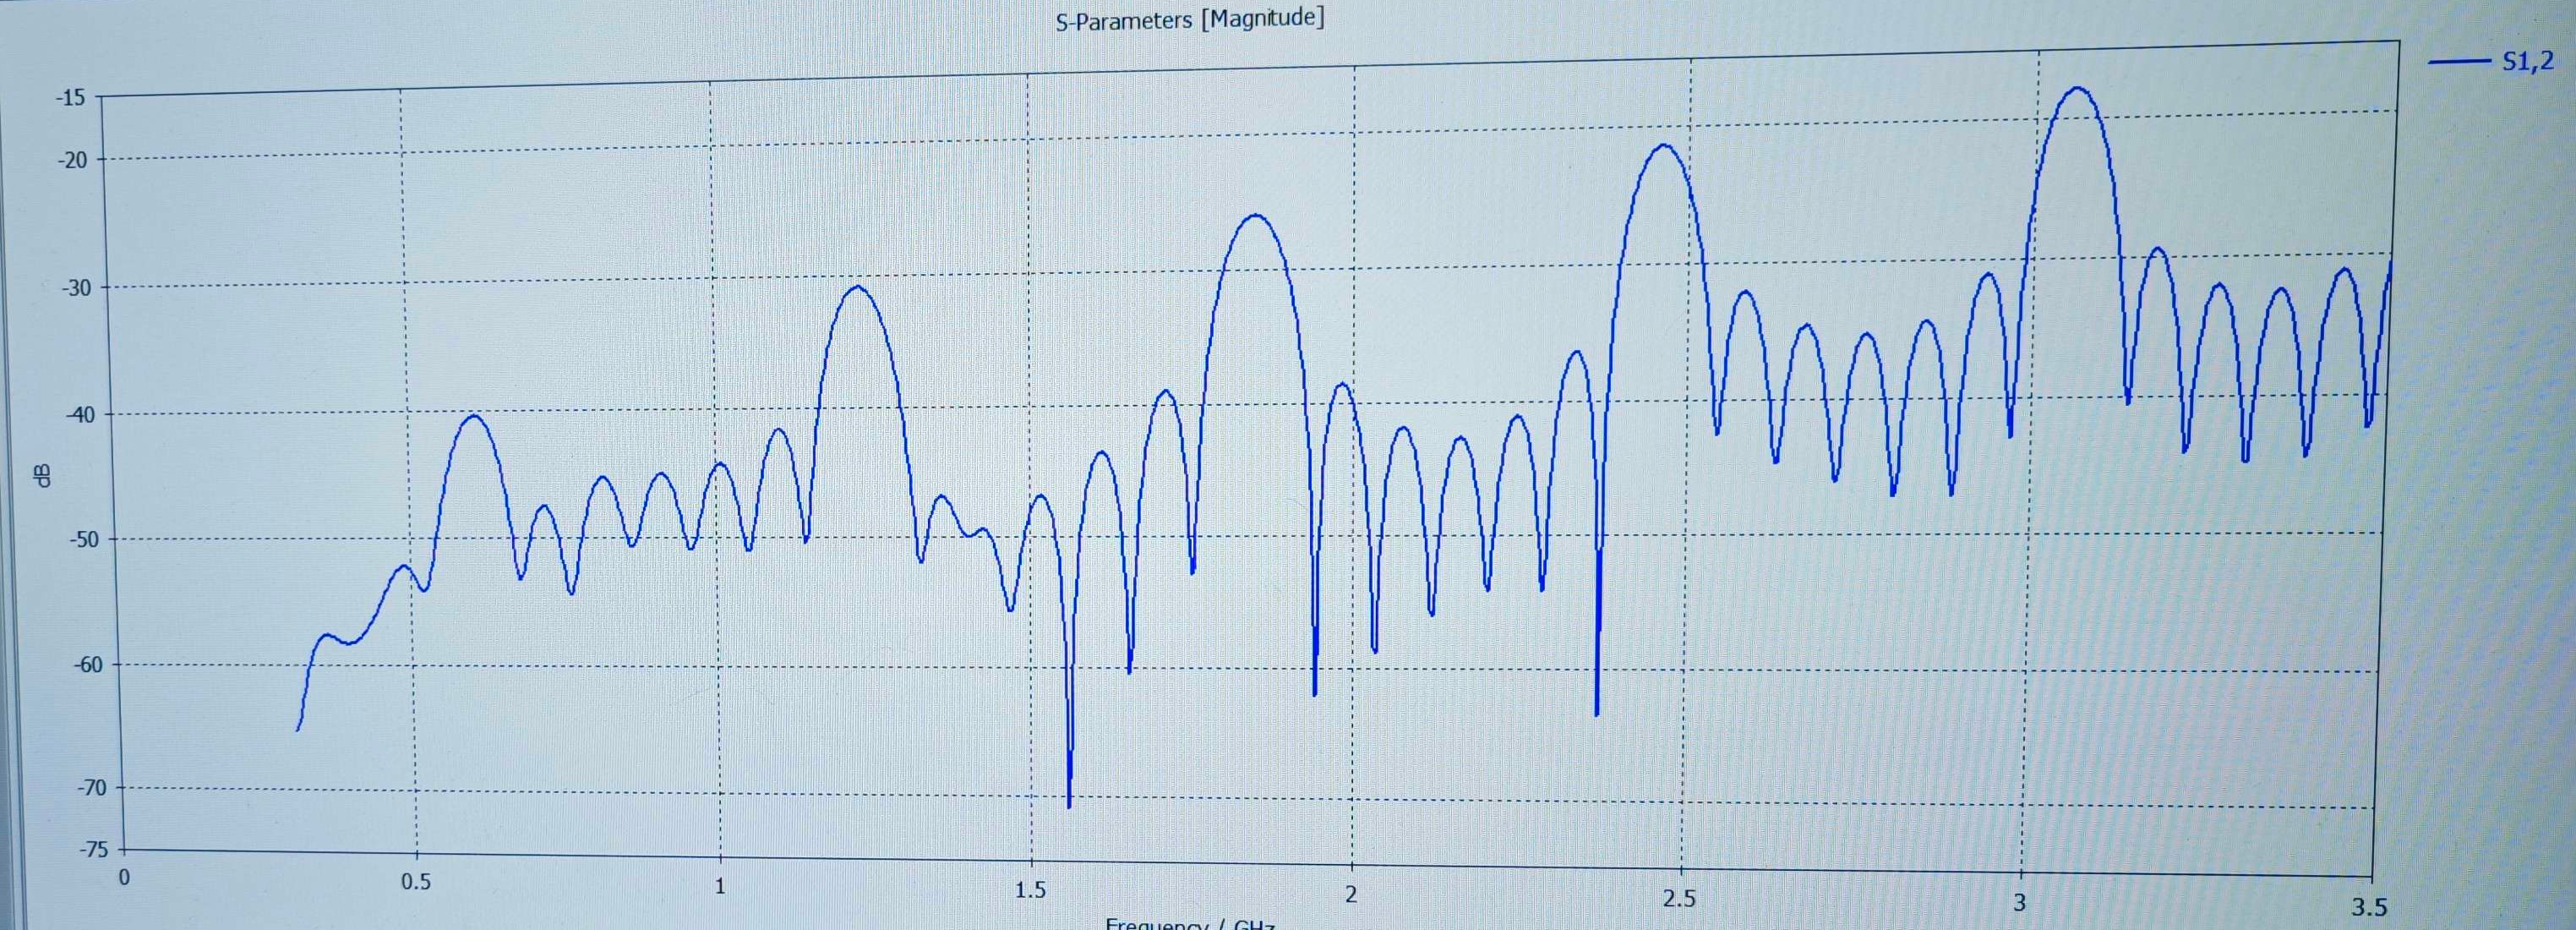
\includegraphics[width=.9\textwidth]{Figures/Lab Four/Resonator_S12.jpg}
  \caption{Resonator $S_{12}$ Plot}
  \label{fig:14}
\end{figure}

\begin{figure}[H]
  \centering
  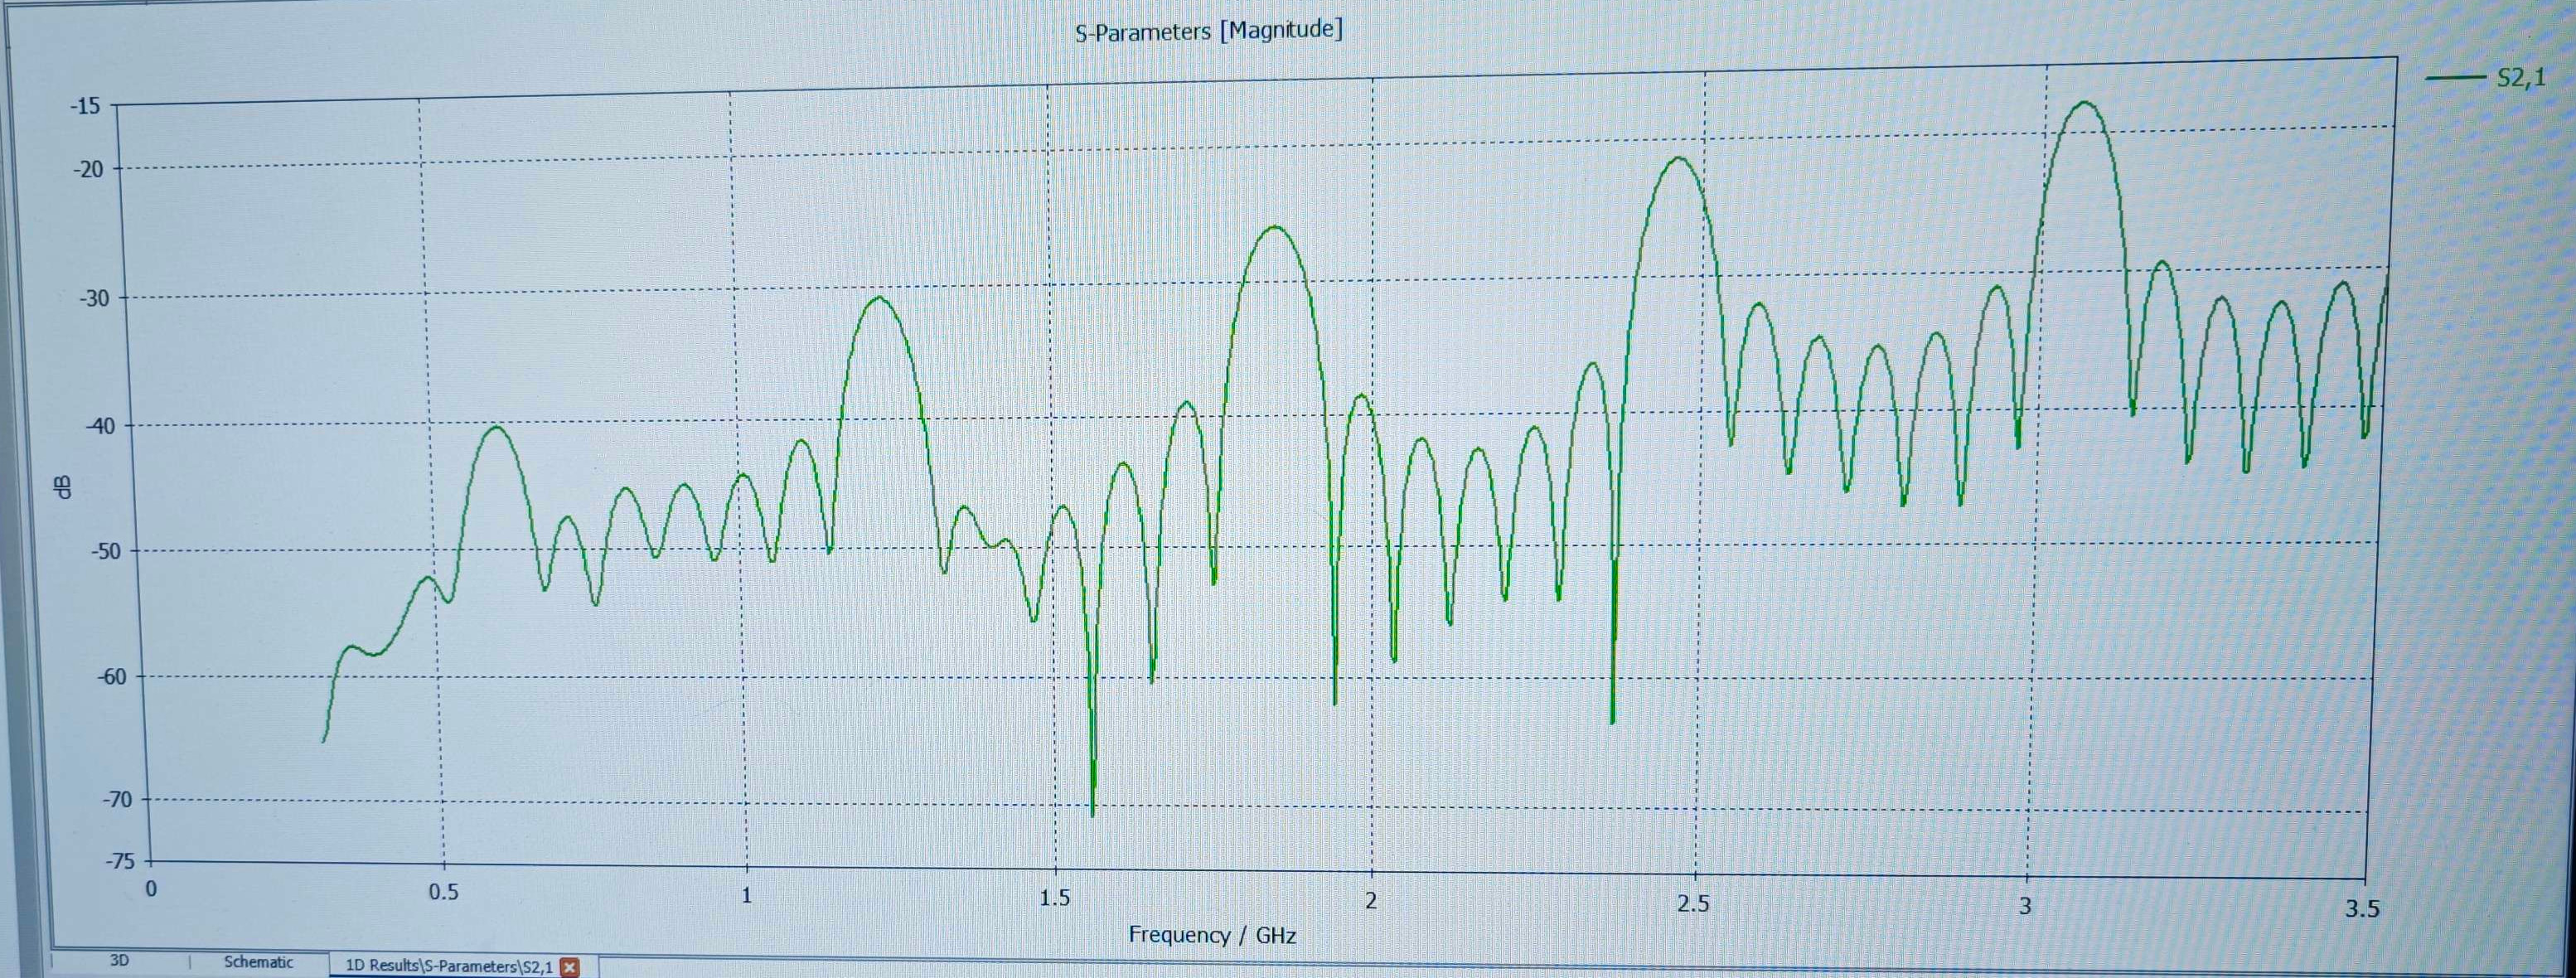
\includegraphics[width=.9\textwidth]{Figures/Lab Four/Resonator_S21.jpg}
  \caption{Resonator $S_{21}$ Plot}
  \label{fig:15}
\end{figure}

\begin{figure}[H]
  \centering
  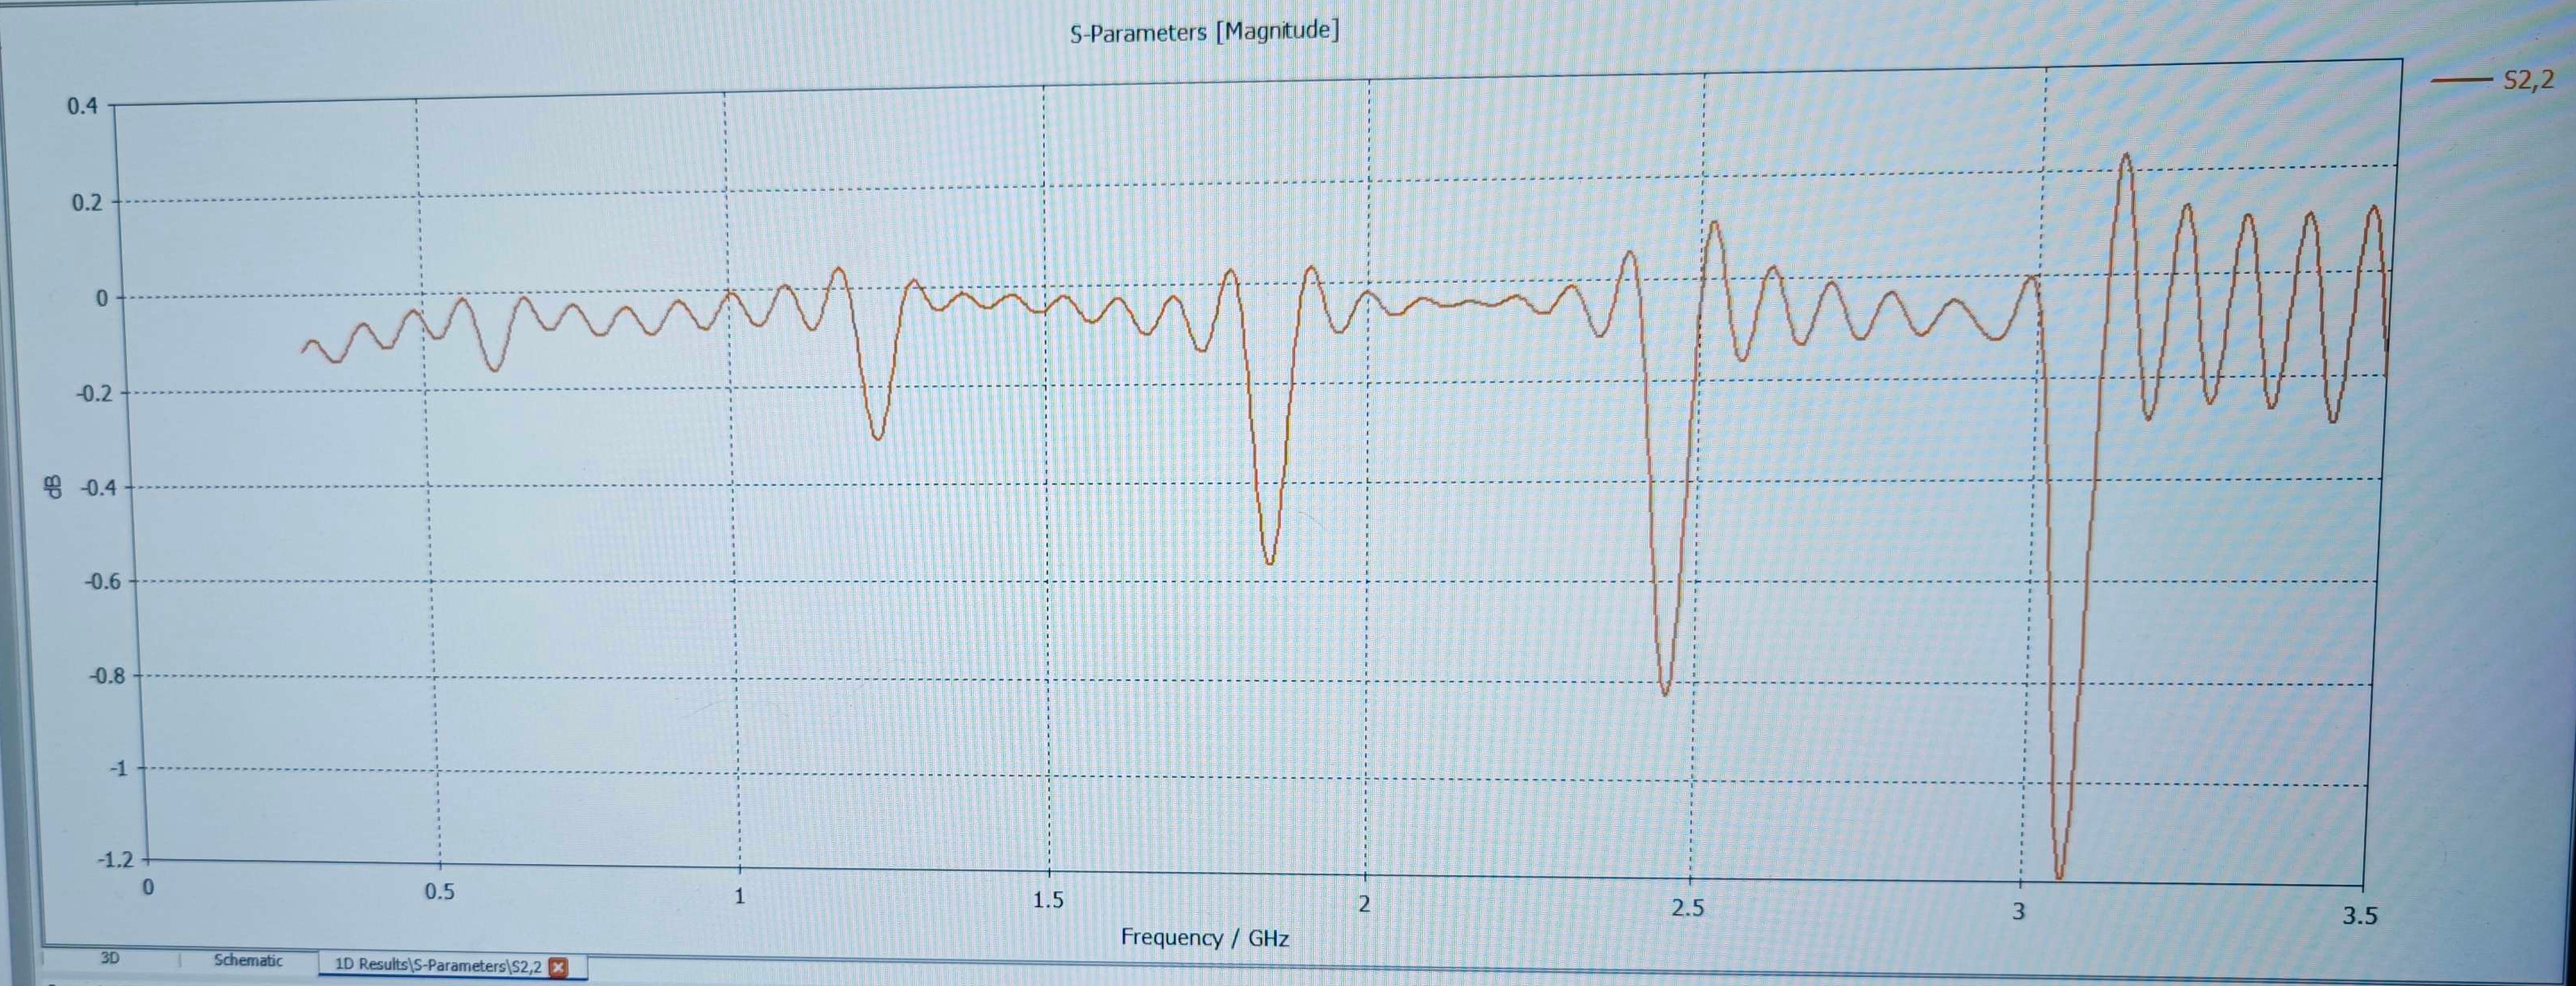
\includegraphics[width=.9\textwidth]{Figures/Lab Four/Resonator_S22.jpg}
  \caption{Resonator $S_{22}$ Plot}
  \label{fig:16}
\end{figure}

\begin{figure}[H]
  \centering
  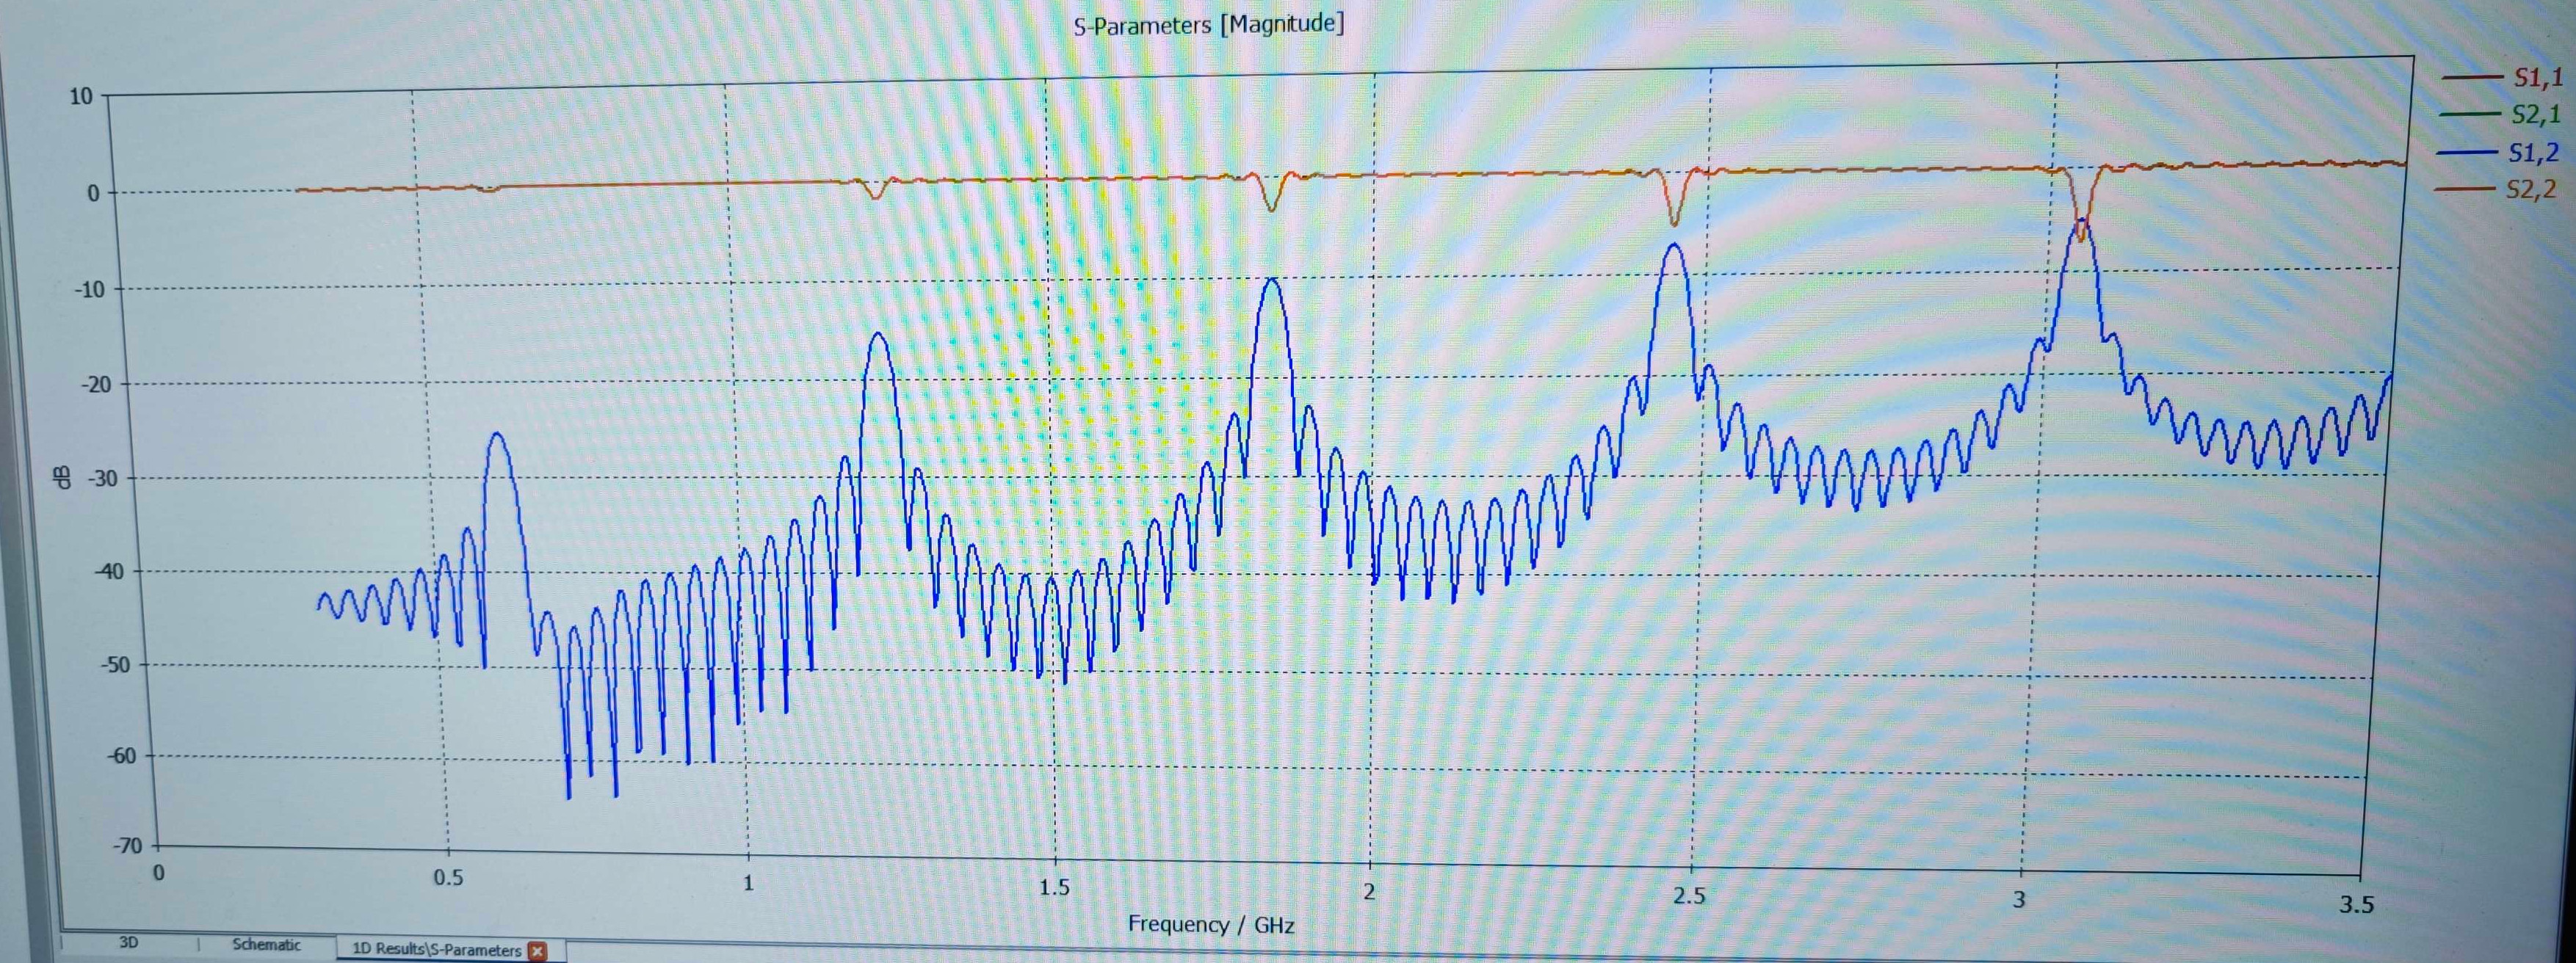
\includegraphics[width=.9\textwidth]{Figures/Lab Four/Resonator_S11_S22.jpg}
  \caption{Resonator $S_{11}$ and $S_{22}$ Plot for Gap of $1[\si{\milli\meter}]$}
  \label{fig:17}
\end{figure}

\section{Conclusion}

\subsection{Questions}

\begin{enumerate}

  \item Explain the definition of $S$ parameters and what kinds of information can be obtained from $S$ parameters.

    $S$ parameters, or scattering parameters, are used to analyze the movement of energy through a system. More specifically, $S$ parameters analyze the differences in voltage and current at high frequency in different ports. The $S$ parameters for a two-port system can be defined as the input voltage reflection coefficient ($\Gamma_i\to S_{11}$), the voltage gain in the reverse direction ($S_{12}$), the voltage gain in the forward direction ($S_{21}$), and the output reflection coefficient ($S_{22}$). Taken as a square matrix, these values can be used to calculate many other important values for an electrical network, for example, the standing wave ratio.

  \item How do meshes work in simulation and why are they important? How to increase the accuracy and resolution of simulated results and what are the potential issues.

    Three-dimensional rendering software generally uses meshes to define shapes. Essentially, geometric shapes are constructed with much smaller shapes. These much smaller shapes are known as the ``mesh.'' Essentially, the higher quality a mesh is (or the more of these smaller shapes used to fill in a geometry) the more accurate the results produced from a simulation. Meshing is the process by which a mesh is generated to fill a shape using a discrete size. Once defined by meshes, simulations may be run; however, the higher quality a mesh is, the more repetitive calculations need to be run, thus requiring greater compute power. This means that, when the accuracy and resolution is increased, processing times are increased, as more calculations need to be performed.

  \item What is the eigenmode of a transmission line or a waveguide.

    The eigenmode is used to run extensive simulations on electromagnetic propagation. Both the electric and magnetic fields are decomposed into eigenmodes, or cross-sections of the constructed device. Two modes, guided and radiated, are combined to form a full eigenmode set. The matrix of $S$ parameters is then applied to generate results for a simulation.

  \item How do the material properties such as the permittivity and conductivities affect the simulation results of a transmission line.

    We know from our definitions that:

    $$\varepsilon_c=\varepsilon-\frac{j\sigma}{\omega}$$

    Furthermore, we know that, when the conductivity decreases, the material becomes an insulator with $\varepsilon_c=\varepsilon$. Thus, with a lower conductivity, more signal attenuation will occur. Additionally, we know that, with a higher dielectric permittivity, there will be a similar effect. Thus, a simulation would have greater signal attenuation with lower conductivity and greater permittivity.

  \item Observe the 1D, 2D and 3D simulation results and describe what information can be obtained from those results.

    Using the unidimensional simulations, we are able to correctly obtain the $S$ parameters of the device. Using the multidimensional simulations, we are able to accurately model the electromagnetic fields along the device.

  \item Show the S-parameters of resonators with different gap size. Comment the variations you see.

    Throughout the experiment, we discovered that a higher gap size corresponds to a lower magnitude of the scattering parameters.

  \item Choose a gap-size value and observe the electric field intensity distribution at resonant wavelength and at non-resonant wavelength and describe the difference. Include figures in your report.

    At resonant frequencies, the magnitude of the $S$ parameters is maximized, thus yielding a more intense electric field. On the other hand, using non-resonant frequencies decreases the magnitude, which then results in a less intense electric field. Figures \ref{fig:13}-\ref{fig:17} show the results for a gap size of $1[\si{\milli\meter}]$.

  \item Change material. Try FR4, Rogers. Which differences you see? (s-parameters, electric field)

    FR4, Rogers has a higher dielectric constant. This allows for greater $S$ parameters, thus yielding a more intense electric field.

  \item Try to make the transmission line wider. Do you see any variations on the $Q$?

    With a wider transmission line, we obtained a greater bandwidth. This resulted in a smaller $Q$ value.

\end{enumerate}

\subsection{Summary}

Overall, with this laboratory experiment, we were successfully able to familiarize ourselves with the use of CST Studio Suite for electrical simulations. We generated plots for the $S$ parameters, as well as various displays used to analyze the electric and magnetic fields in different dimensions.

\end{document}
